% !TEX program = xelatex
% !TeX spellcheck = ru_RU_yo

\documentclass[xetex,t]{beamer}

\usepackage{xecyr}
\usepackage{xunicode}
\usepackage{fontspec}
\defaultfontfeatures{Ligatures=TeX}
\setmainfont{ALSSchlangesans}

\usepackage{polyglossia}
\setdefaultlanguage[spelling=modern]{russian}
\newfontfamily{\cyrillicfont}[BoldFont={*-Bold}]{ALSSchlangesans}
\newfontfamily{\cyrillicfontsf}[BoldFont={*-Bold}]{ALSSchlangesans}
\newfontfamily{\cyrillicfonttt}{Droid Sans Mono}

\usepackage[euler-digits,small]{eulervm}
\AtBeginDocument{\renewcommand{\hbar}{\hslash}}

\definecolor{ifmoblue}{RGB}{25,70,186}
\definecolor{ifmored}{RGB}{236,11,67}

\setbeamertemplate{itemize items}[circle]

\usepackage{epstopdf}
\usepackage{graphicx}
\usepackage{amsmath}
\usepackage{nicefrac}
\usepackage{ctable}
\usepackage{ragged2e}

\usepackage{pifont}
\newcommand{\cmark}{\ding{51}}%
\newcommand{\xmark}{\ding{55}}%


\usepackage{xcolor}
\newcommand{\highlight}[1]{\colorbox{orange!50}{$\displaystyle#1$}}

\usepackage{textpos}

\newcommand{\email}[1]{{\scriptsize\texttt{#1}}}

\usebackgroundtemplate{}

\titlegraphic{
\includegraphics[width=5cm]{ifmo/logo-blue}}
\title{Разработка веб-приложения для работы\\с программным пакетом высокоточного позиционирования RTKLIB}
\author[Кузнецов А.А., P3410]{Кузнецов Андрей Андреевич, ФПИиКТ, ИПМ, Р4215}
\date[]{Научный руководитель: Соснин В.В., к.т.н., доцент}

\usetheme{ifmo}
\setbeamersize{text margin left=0.6cm,text margin right=0.5cm}

\begin{document}

%
% Title
%
\begin{frame}
  \titlepage
\end{frame}


%
% DGPS
%
\begin{frame}
  \frametitle{Дифференциальная GPS}

  \only<1>{
    \begin{center}
      \textbf{Дифференциальная GPS} (англ. \emph{Differential Global Positioning System}) -- система, предназначенная для повышения точности сигналов GPS. Принцип работы данной системы заключается в~измерении и~учёте разницы между рассчитанной и~закодированной псевдодальностями до спутников.
    \end{center}
    
    \vskip -0.25cm
    
    \begin{figure}[h]
      \centering
      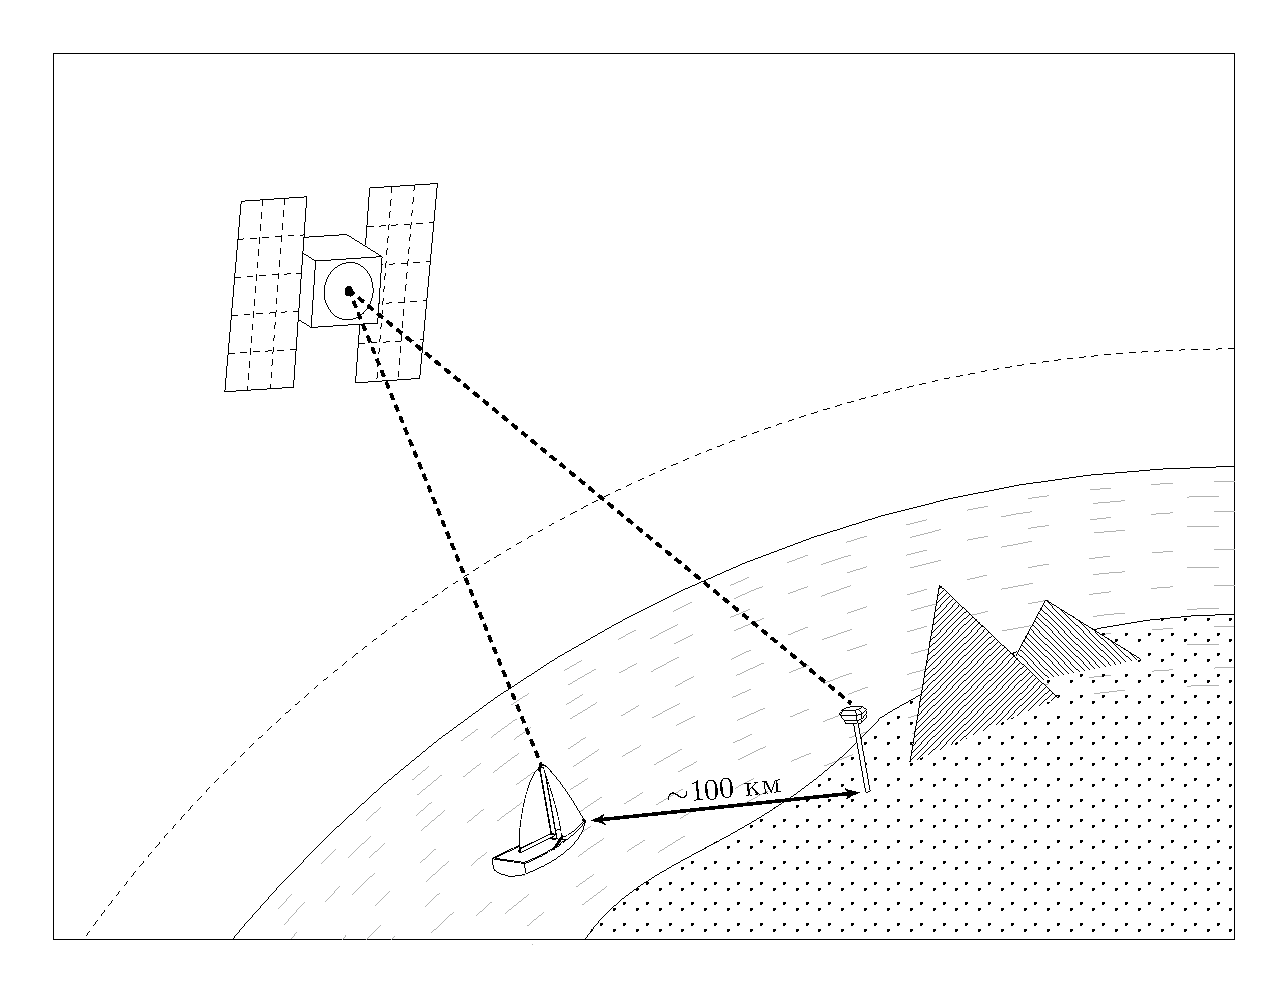
\includegraphics[height=4.5cm]{../img/tikz/dgps-one/pic}
    \end{figure}
  }

  \only<2>{
    \begin{figure}[t]
      \centering
      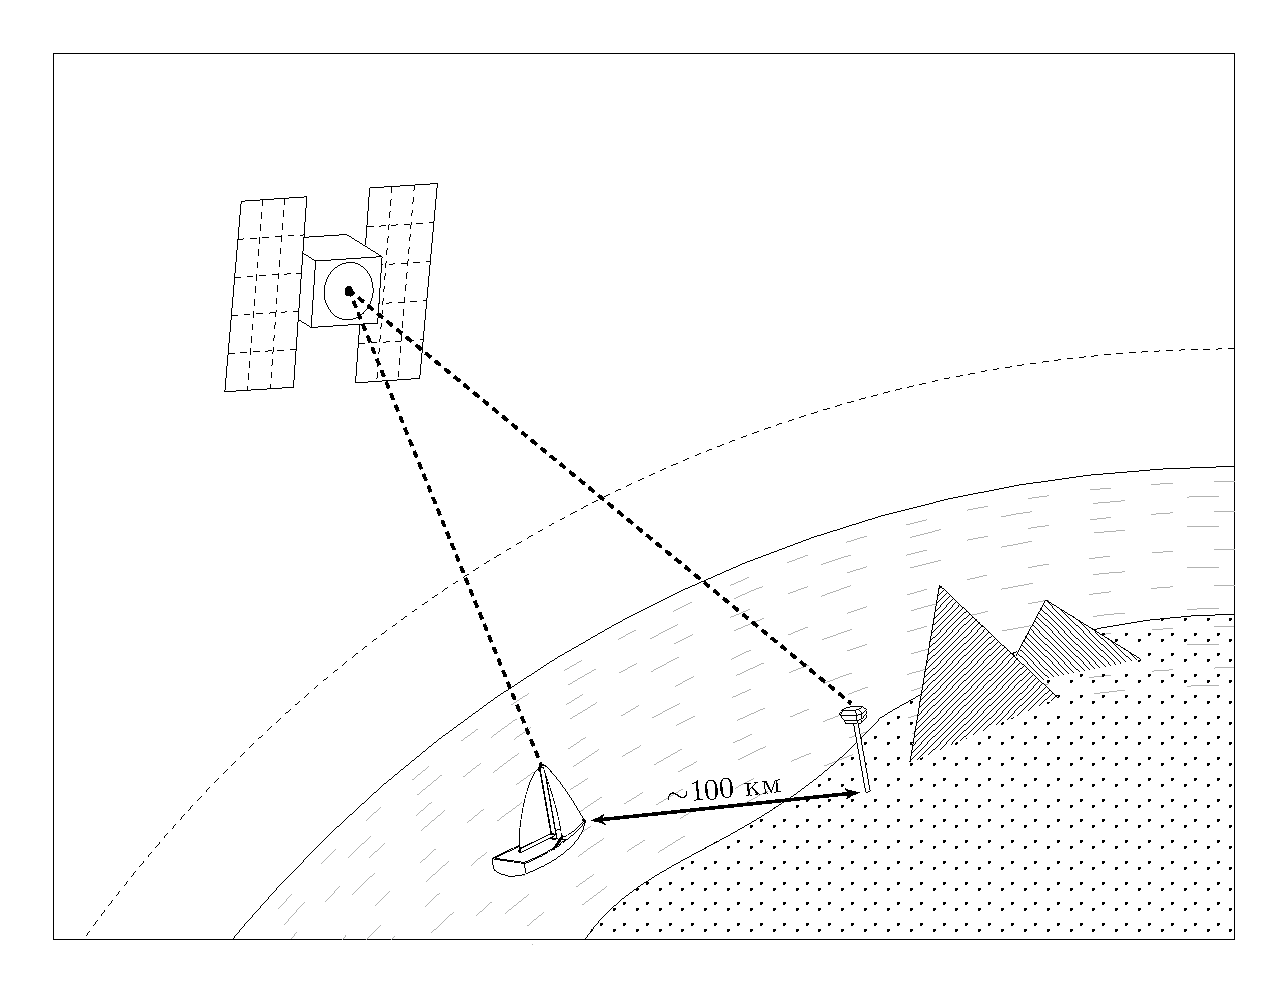
\includegraphics[height=7.25cm]{../img/tikz/dgps-one/pic}
    \end{figure}
  }
\end{frame}


%
% RTK
%
\begin{frame}
  \frametitle{Кинематика реального времени}

  \begin{center}
    \textbf{Кинематика реального времени} (англ. \emph{Real Time Kinematic, RTK}) -- режим работы, при котором приём и~применение поправок с~базы происходят в~реальном времени, что позволяет получать результат практически сразу. Важнейшей особенностью данного режима является тот факт, что для обеспечения работы необходима постоянная связь между ровером и~базой.
  \end{center}

  \vskip 0.25cm

  \only<2>{
    \begin{minipage}{\textwidth}
      \centering
      \begin{minipage}[t]{.3\textwidth}
        \centering
        \begin{figure}[h]
          \centering
          
\includegraphics[height=21pt]{../img/trimble}
        \end{figure}
        \$~10$\,$000

        {
          \scriptsize
          \color{gray}{Trimble R8 Model 3 (2009)}
        }
      \end{minipage}
      \hspace{1em}
      \begin{minipage}[t]{.3\textwidth}
        \centering
        \begin{figure}[h]
          \centering
          
\includegraphics[height=21pt]{../img/leica}
        \end{figure}
        \$~6$\,$000

        {
          \scriptsize
          \color{gray}{Leica Viva GS08 (2012)}
        }
      \end{minipage}
    \end{minipage}
  }
\end{frame}


%
% RTKLIB
%
\begin{frame}
  \frametitle{RTKLIB}
  
  \begin{center}
    \textbf{RTKLIB} -- программный пакет с~открытым исходным кодом, предназначенный для осуществления стандартного и~высокоточного позиционирования с~помощью глобальных навигационных спутниковых систем.
  \end{center}
  
  \begin{figure}[h]
    \centering
    
\includegraphics[height=2cm]{../img/rtklib}
  \end{figure}
\end{frame}


%
% RTKLIB problems
%
\begin{frame}
  \frametitle{RTKLIB}
  \framesubtitle{Проблемы использования}

  \begin{figure}[h]
    \centering
    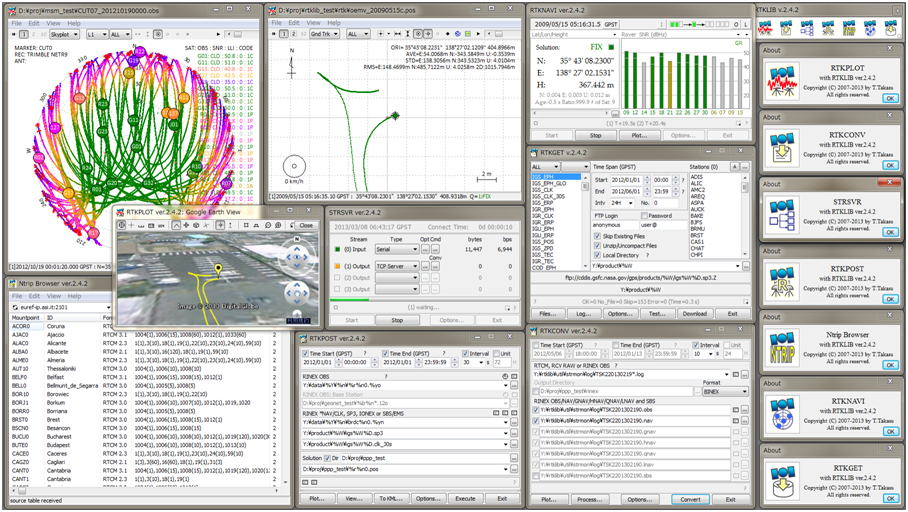
\includegraphics[width=.95\textwidth]{../img/rtklib-hell}
  \end{figure}
\end{frame}


%
% Main task
%
\begin{frame}
  \frametitle{Характеристика проведённой работы}
  \vskip 0.5cm
  \begin{center}
    {
      \Large
      \textbf{Предмет исследования} -- процесс взаимодействия пользователя с~программными компонентами\\пакета RTKLIB.
      \vskip .75cm
      \textbf{Цель работы} -- создание приложения,\\позволяющего взаимодействовать с~RTKLIB\\[0.25em]через веб-браузер.
    }
  \end{center}
\end{frame}


%
% Receivers review
%
\begin{frame}
  \frametitle{Обзор существующих решений}
  \framesubtitle{Интерфейсы для управления приёмниками}

  \begin{textblock*}{3cm}(0.5cm,0.5cm)
    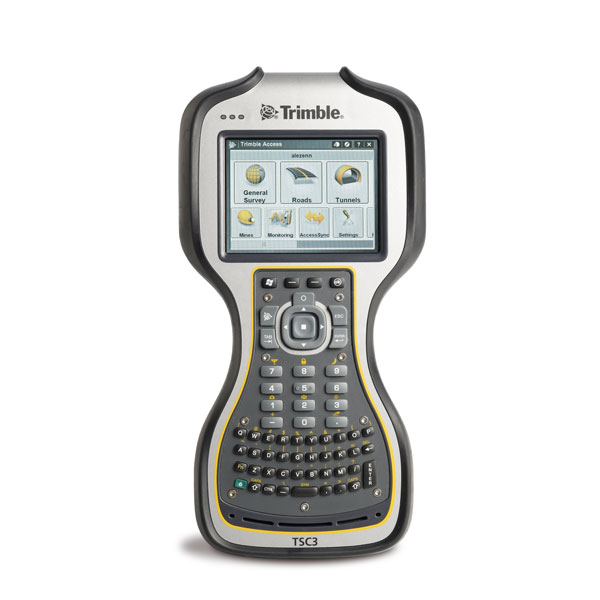
\includegraphics[width=\textwidth]{../img/trimble-tsc3}
  \end{textblock*}
  \begin{textblock*}{3cm}(2cm,4.5cm)
    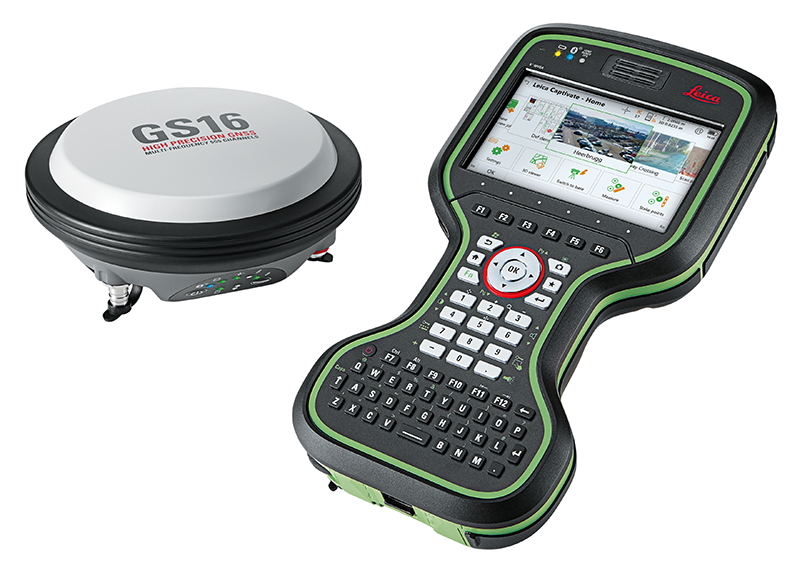
\includegraphics[width=\textwidth]{../img/leica-gs16}
  \end{textblock*}
  \begin{textblock*}{1.5cm}(5.5cm,1cm)
    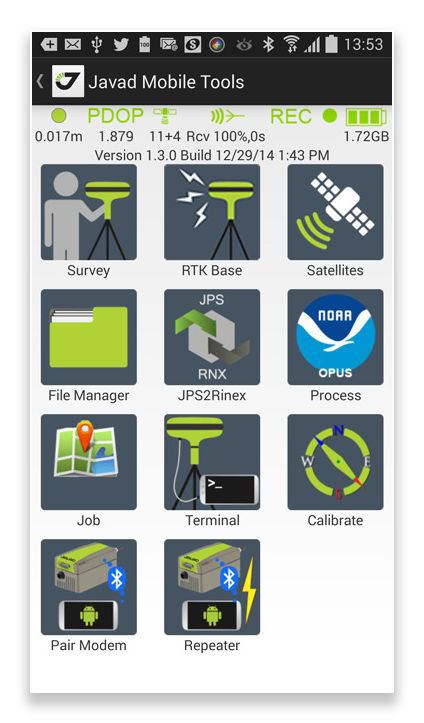
\includegraphics[width=\textwidth]{../img/javad-mobile-tools}
  \end{textblock*}
  \begin{textblock*}{3cm}(4cm,1.5cm)
    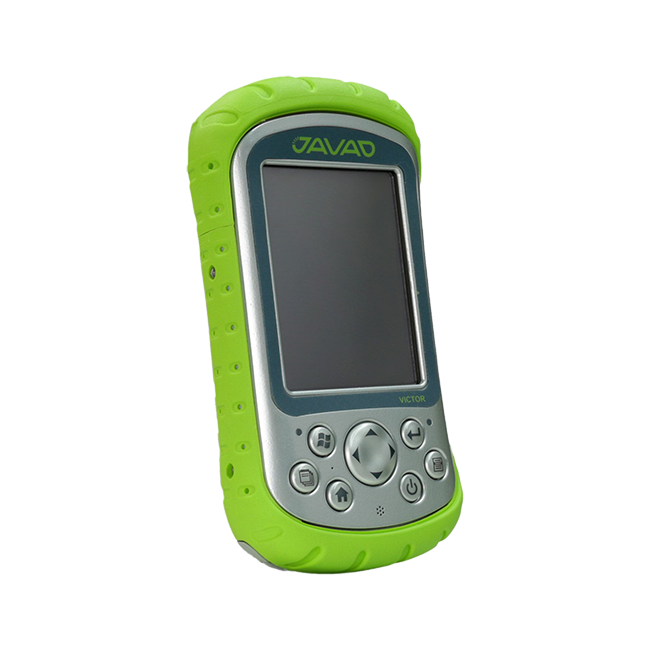
\includegraphics[width=\textwidth]{../img/javad-victor}
  \end{textblock*}
  \begin{textblock*}{3.5cm}(7.75cm,0.5cm)
    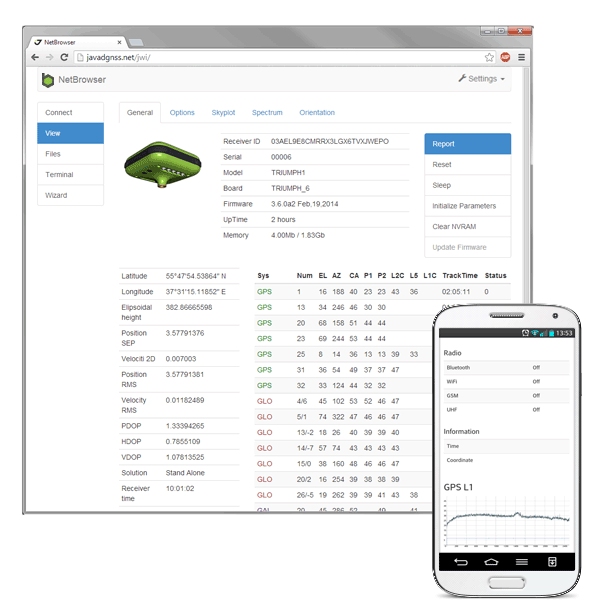
\includegraphics[width=\textwidth]{../img/javad-netbrowser}
  \end{textblock*}
  \begin{textblock*}{1.75cm}(7.25cm,4cm)
    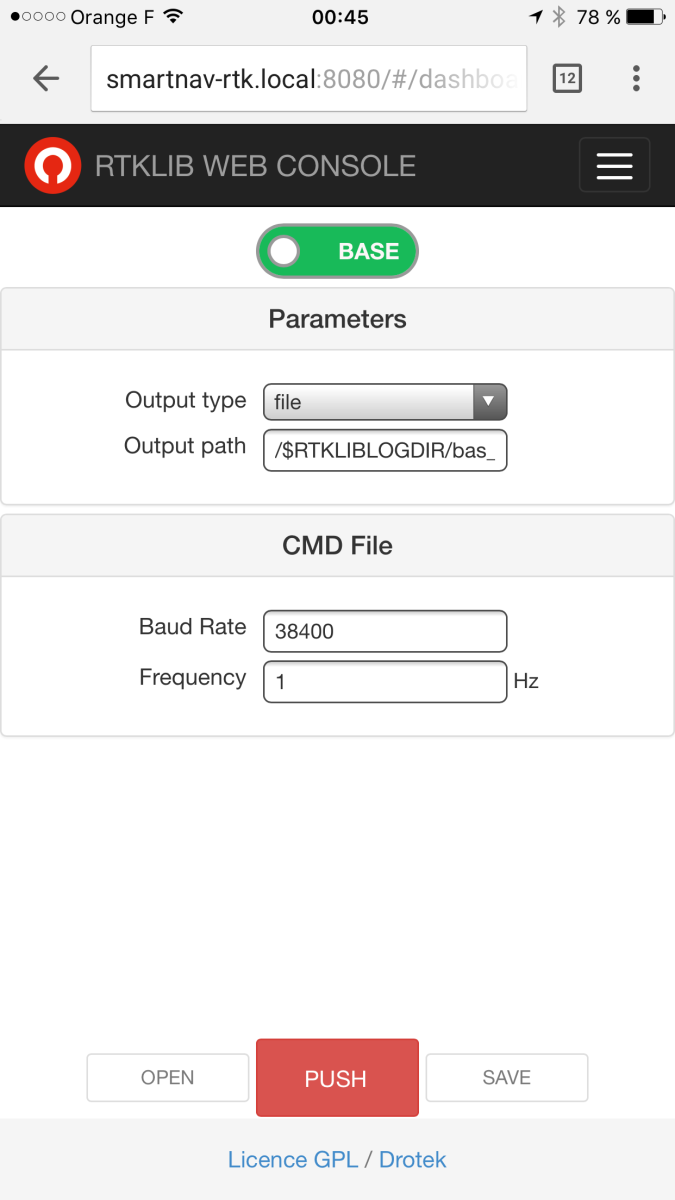
\includegraphics[width=\textwidth]{../img/drotek-web}
  \end{textblock*}
\end{frame}


%
% Web apps review
%
\begin{frame}
  \frametitle{Обзор существующих решений}
  \framesubtitle{Веб-интерфейсы для управления устройствами}
  \vskip 1cm
  \begin{minipage}{\textwidth}
    \centering
    \begin{minipage}[c]{.45\textwidth}
      \centering
      \begin{figure}[h]
        \centering
        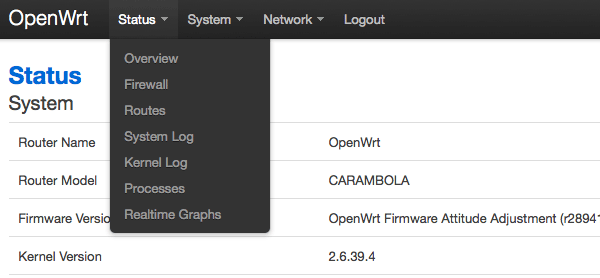
\includegraphics[width=\textwidth]{../img/openwrt-menu}
      \end{figure}
      OpenWrt
    \end{minipage}
    \hspace{1em}
    \begin{minipage}[c]{.45\textwidth}
      \centering
      \begin{figure}[h]
        \centering
        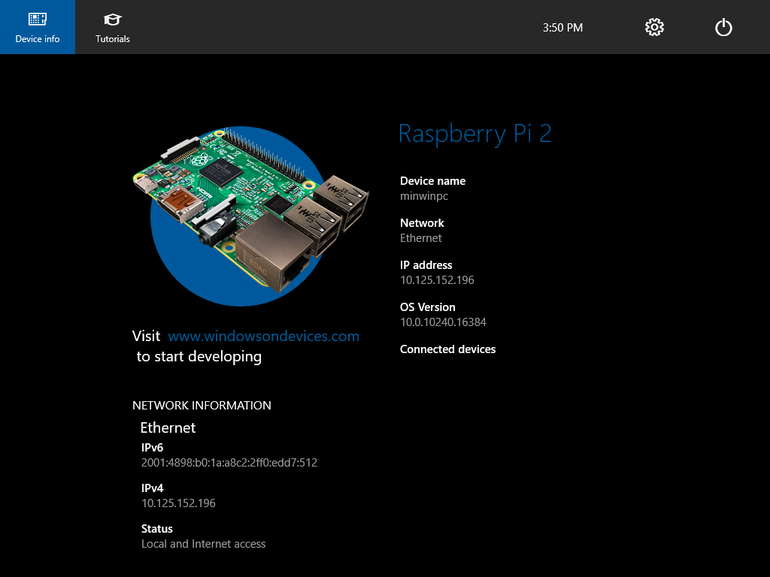
\includegraphics[width=\textwidth]{../img/win10-device-info}
      \end{figure}
      Windows 10 IoT Core
    \end{minipage}
  \end{minipage}
\end{frame}


%
% Reach & Reach RS
%
\begin{frame}
  \frametitle{Платформа для разработки}
  
  \begin{minipage}{\textwidth}
    \centering
    
\includegraphics[width=.25\textwidth]{../img/emlid-logo}
    \vskip 1.25cm
    \begin{minipage}[c]{.45\textwidth}
      \centering
      \begin{figure}[h]
        \centering
        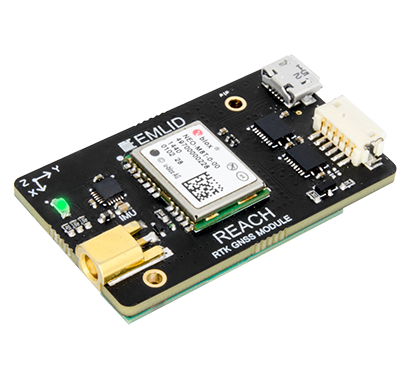
\includegraphics[height=3.5cm]{../img/reach}
      \end{figure}
      Reach
    \end{minipage}
    \hspace{1em}
    \begin{minipage}[c]{.45\textwidth}
      \centering
      \begin{figure}[h]
        \centering
        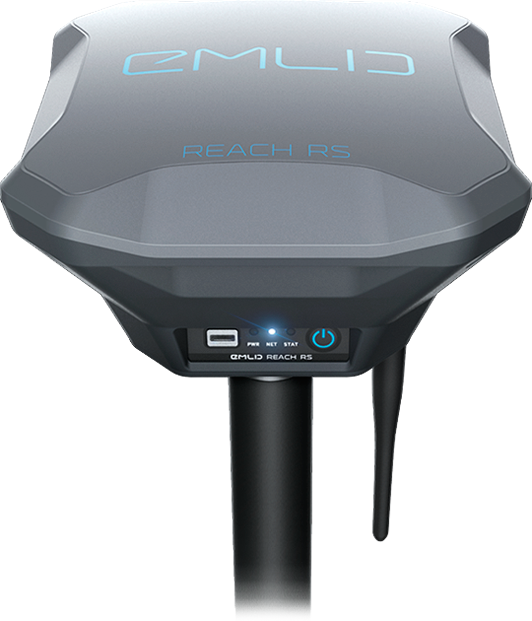
\includegraphics[height=3.5cm]{../img/reach-rs}
      \end{figure}
      Reach RS
    \end{minipage}
  \end{minipage}
\end{frame}


%
% Required features
%
\begin{frame}
  \frametitle{Основные требования к веб-приложению}
  
  \begin{itemize}
    \item Одностраничное приложение
    \item Автоматическая подстройка под тип устройства
    \item Адаптивность и кроссбраузерность
  \end{itemize}
  \begin{center}
    \vskip -0.7cm
    \color{ifmoblue}{\rule{.5\textwidth}{0.5pt}}
  \end{center}
  \vskip -0.5cm
  \begin{itemize}
    \item Отображение информации о~спутниках
    \item Отображение информации в~соответствии с~текущей ролью в~RTK-системе
    \item Настройка RTK и~приёмника
    \item Настройка входных/выходных потоков данных
    \item Доступ к~логам и~их настройкам
    \item Настройка беспроводных интерфейсов
  \end{itemize}
\end{frame}


%
% Raw architecture
%
\begin{frame}
  \frametitle{Общая архитектура приложения}
  \vskip -0.75cm
  \begin{figure}[h]
    \centering
    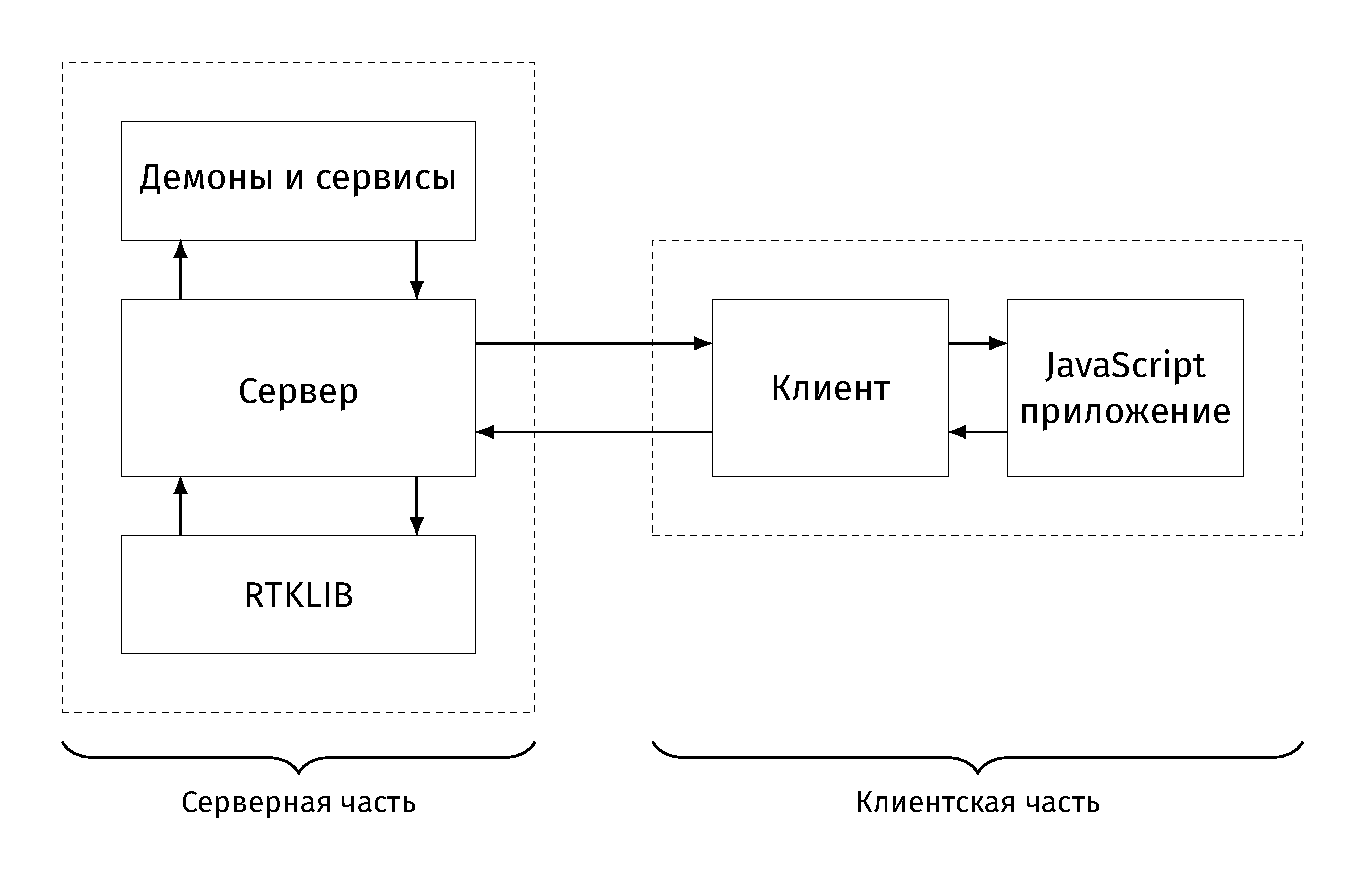
\includegraphics[width=.95\textwidth]{../img/tikz/raw-system-architecture/pic}
  \end{figure}
\end{frame}


%
% Tools
%
\begin{frame}
  \frametitle{Средства разработки}
  {
    \Large
    \begin{itemize}
      \item Python (Flask)
      \item JavaScript (Vue.js + Vuex, D3.js, OpenLayers)
      \item Socket.io (WebSocket)
    \end{itemize}
    
    \begin{itemize}
      \item Karma + Mocha
      \item PyTest + Selenium
    \end{itemize}
  }
\end{frame}


%
% System architecture
%
\begin{frame}
  \frametitle{Общая архитектура приложения}
  \vskip -0.75cm
  \begin{figure}[h]
    \centering
    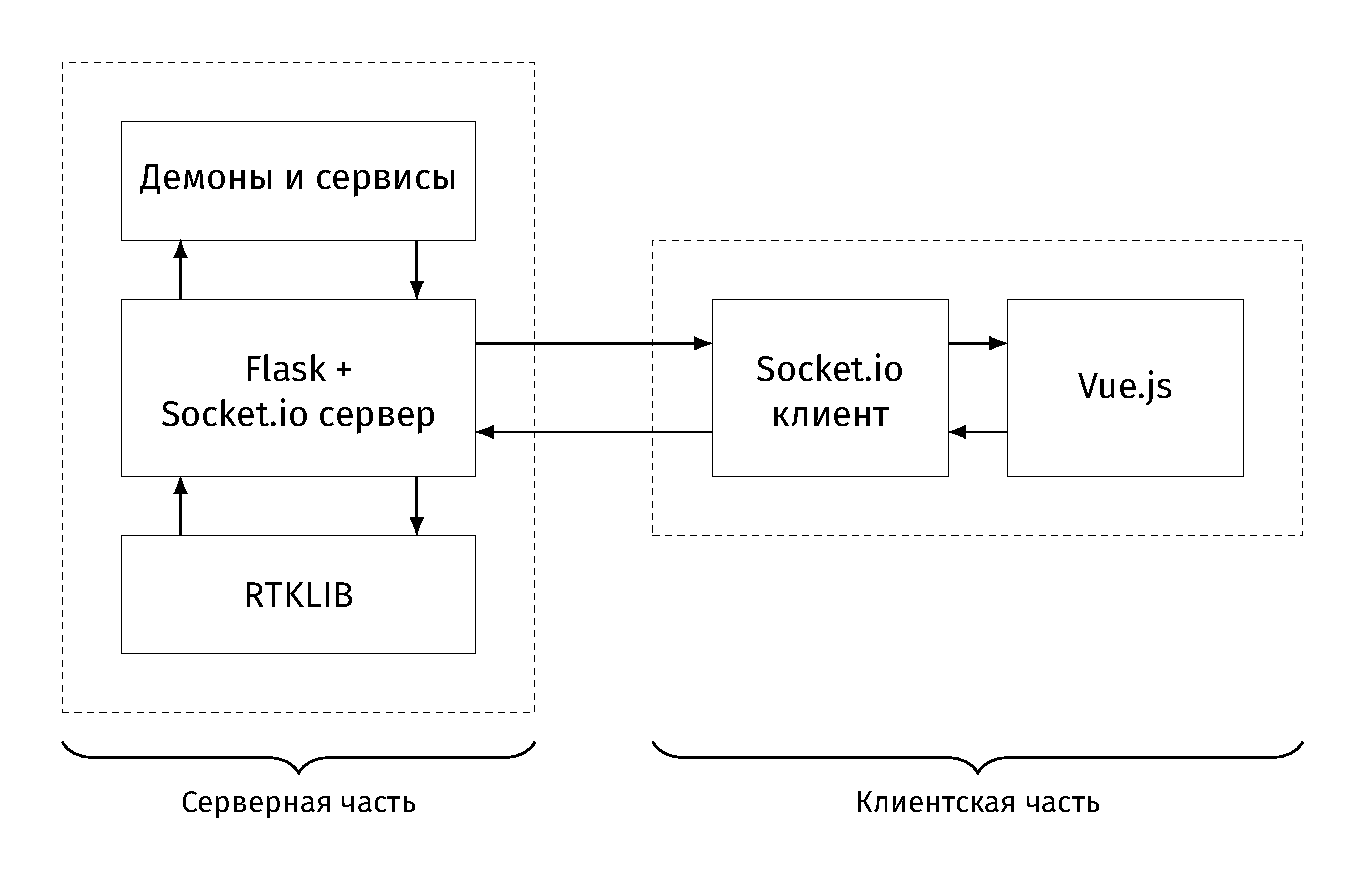
\includegraphics[width=.95\textwidth]{../img/tikz/system-architecture/pic_sans_no-border}
  \end{figure}
\end{frame}


%
% FE architecture
%
\begin{frame}
  \frametitle{Архитектура клиентской части приложения}
\end{frame}


%
% "Home page"
%
\begin{frame}
  \frametitle{Разработка веб-приложения}
  \vskip -0.5cm
  \begin{figure}[h]
    \centering
    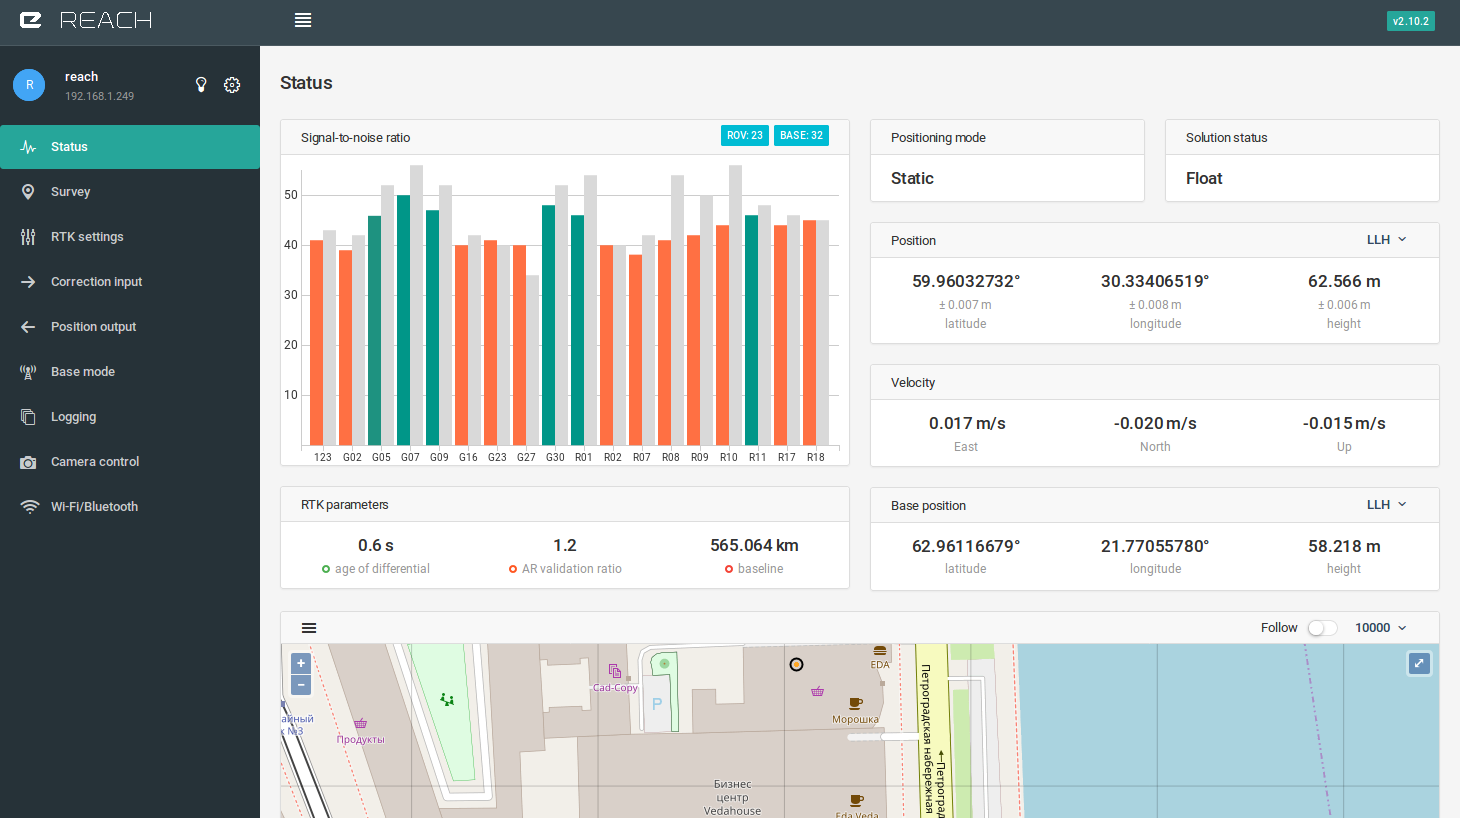
\includegraphics[width=.95\textwidth]{../img/reachview/home}
  \end{figure}
\end{frame}


%
% Responsive UI
%
\begin{frame}
  \frametitle{Разработка веб-приложения}
  \framesubtitle{Адаптивный интерфейс}
  
  \begin{minipage}{\textwidth}
    \centering
    \begin{minipage}[c]{.5\textwidth}
      \centering
      \begin{figure}[c]
        \centering
        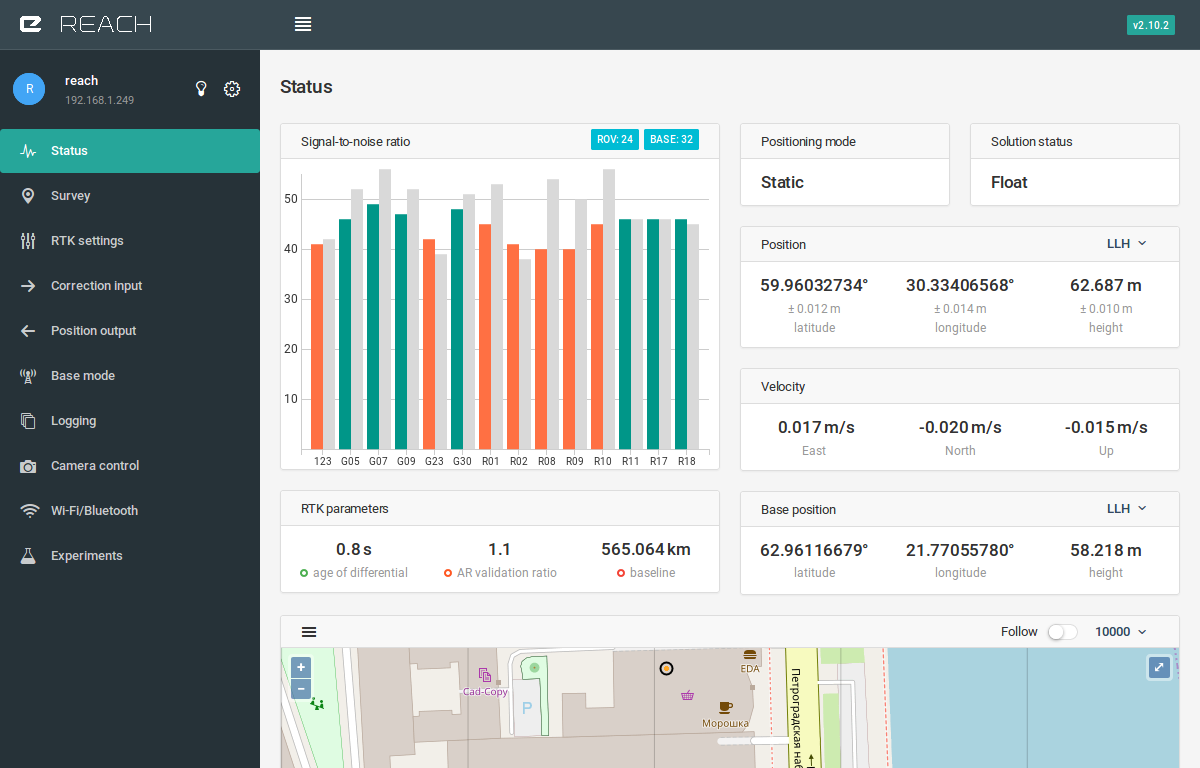
\includegraphics[height=4cm]{../img/reachview/homepage_responsive-lg}
      \end{figure}
    \end{minipage}
    \hspace{2em}
    \begin{minipage}[c]{.3\textwidth}
      \centering
      \begin{figure}[c]
        \centering
        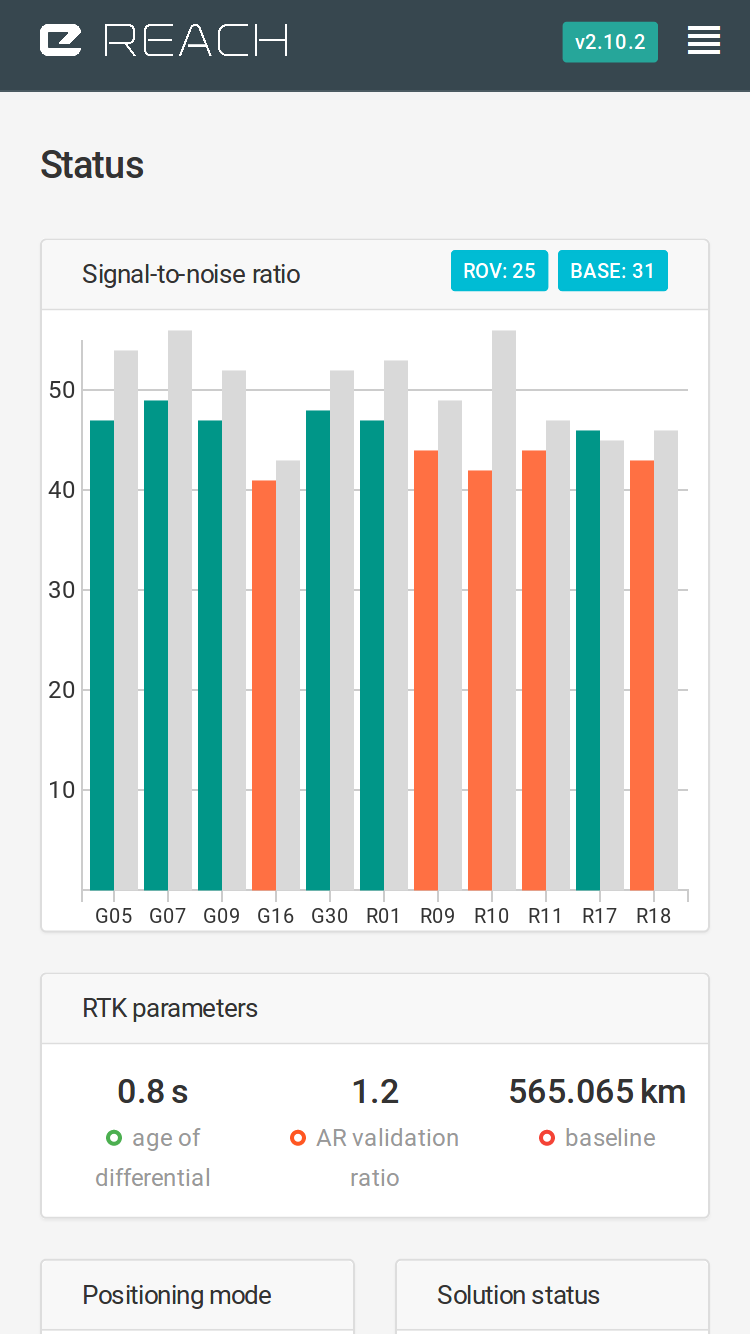
\includegraphics[height=5.5cm]{../img/reachview/homepage_responsive-xs}
      \end{figure}
    \end{minipage}
  \end{minipage}
\end{frame}


\setbeamercovered{transparent}

%
% Tabs
%
\begin{frame}
  \frametitle{Разработка веб-приложения}
  \framesubtitle{Разделение на интерфейса на секции}

  \begin{minipage}[c]{\textwidth}
    \centering
    \footnotesize
    \vskip 0.5cm
    \begin{minipage}[c]{.32\textwidth}
      \begin{itemize}
        \item<1> Статус
        \item<2> Изыскания
        \item<3> Настройки RTK
        \item<4> Входящие поправки
        \item<5> Выдача позиции
        \item<6> Режим базы
        \item<7> Логирование
        \item<8> Управление камерой
        \item<9> Wi-Fi/Bluetooth
        \item<10> Настройки
      \end{itemize}
    \end{minipage}
    \hspace{1em}
    \begin{minipage}[c]{.64\textwidth}
      \only<1>{
        \begin{figure}[c]
          \centering
          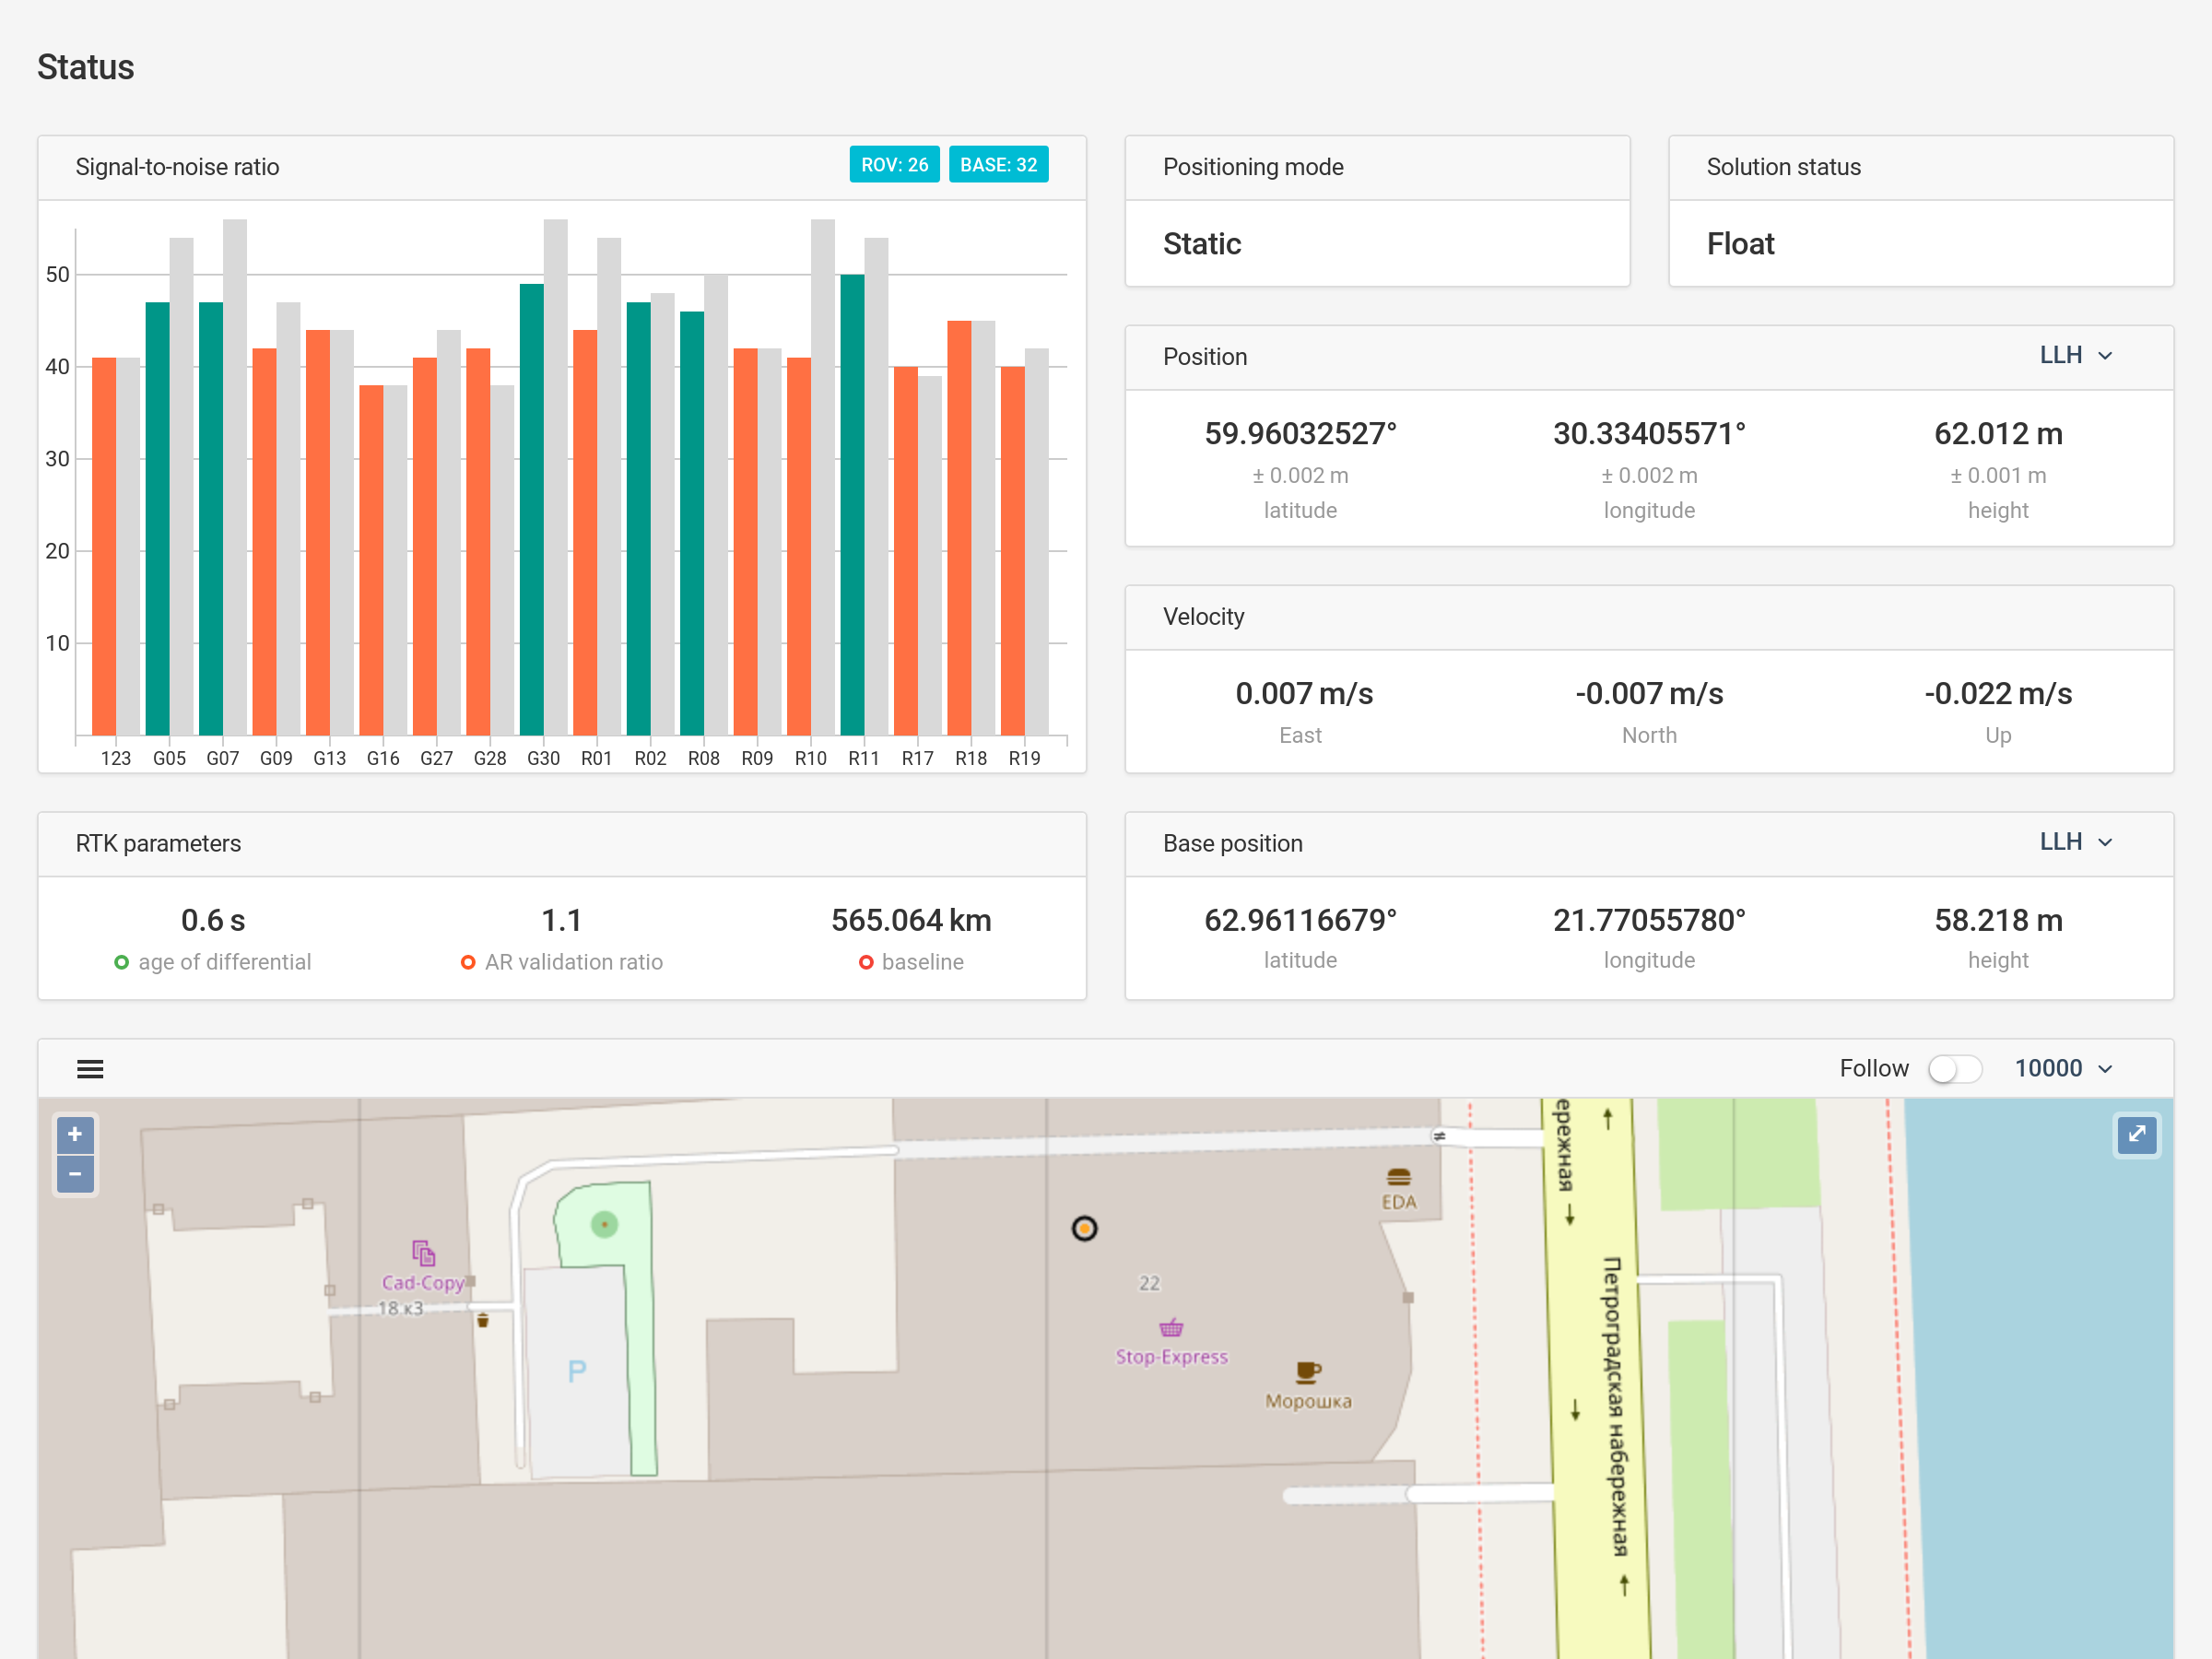
\includegraphics[width=\textwidth]{../img/reachview/status_content_laptop}
        \end{figure}
      }
      \only<2>{
        \begin{figure}[c]
          \centering
          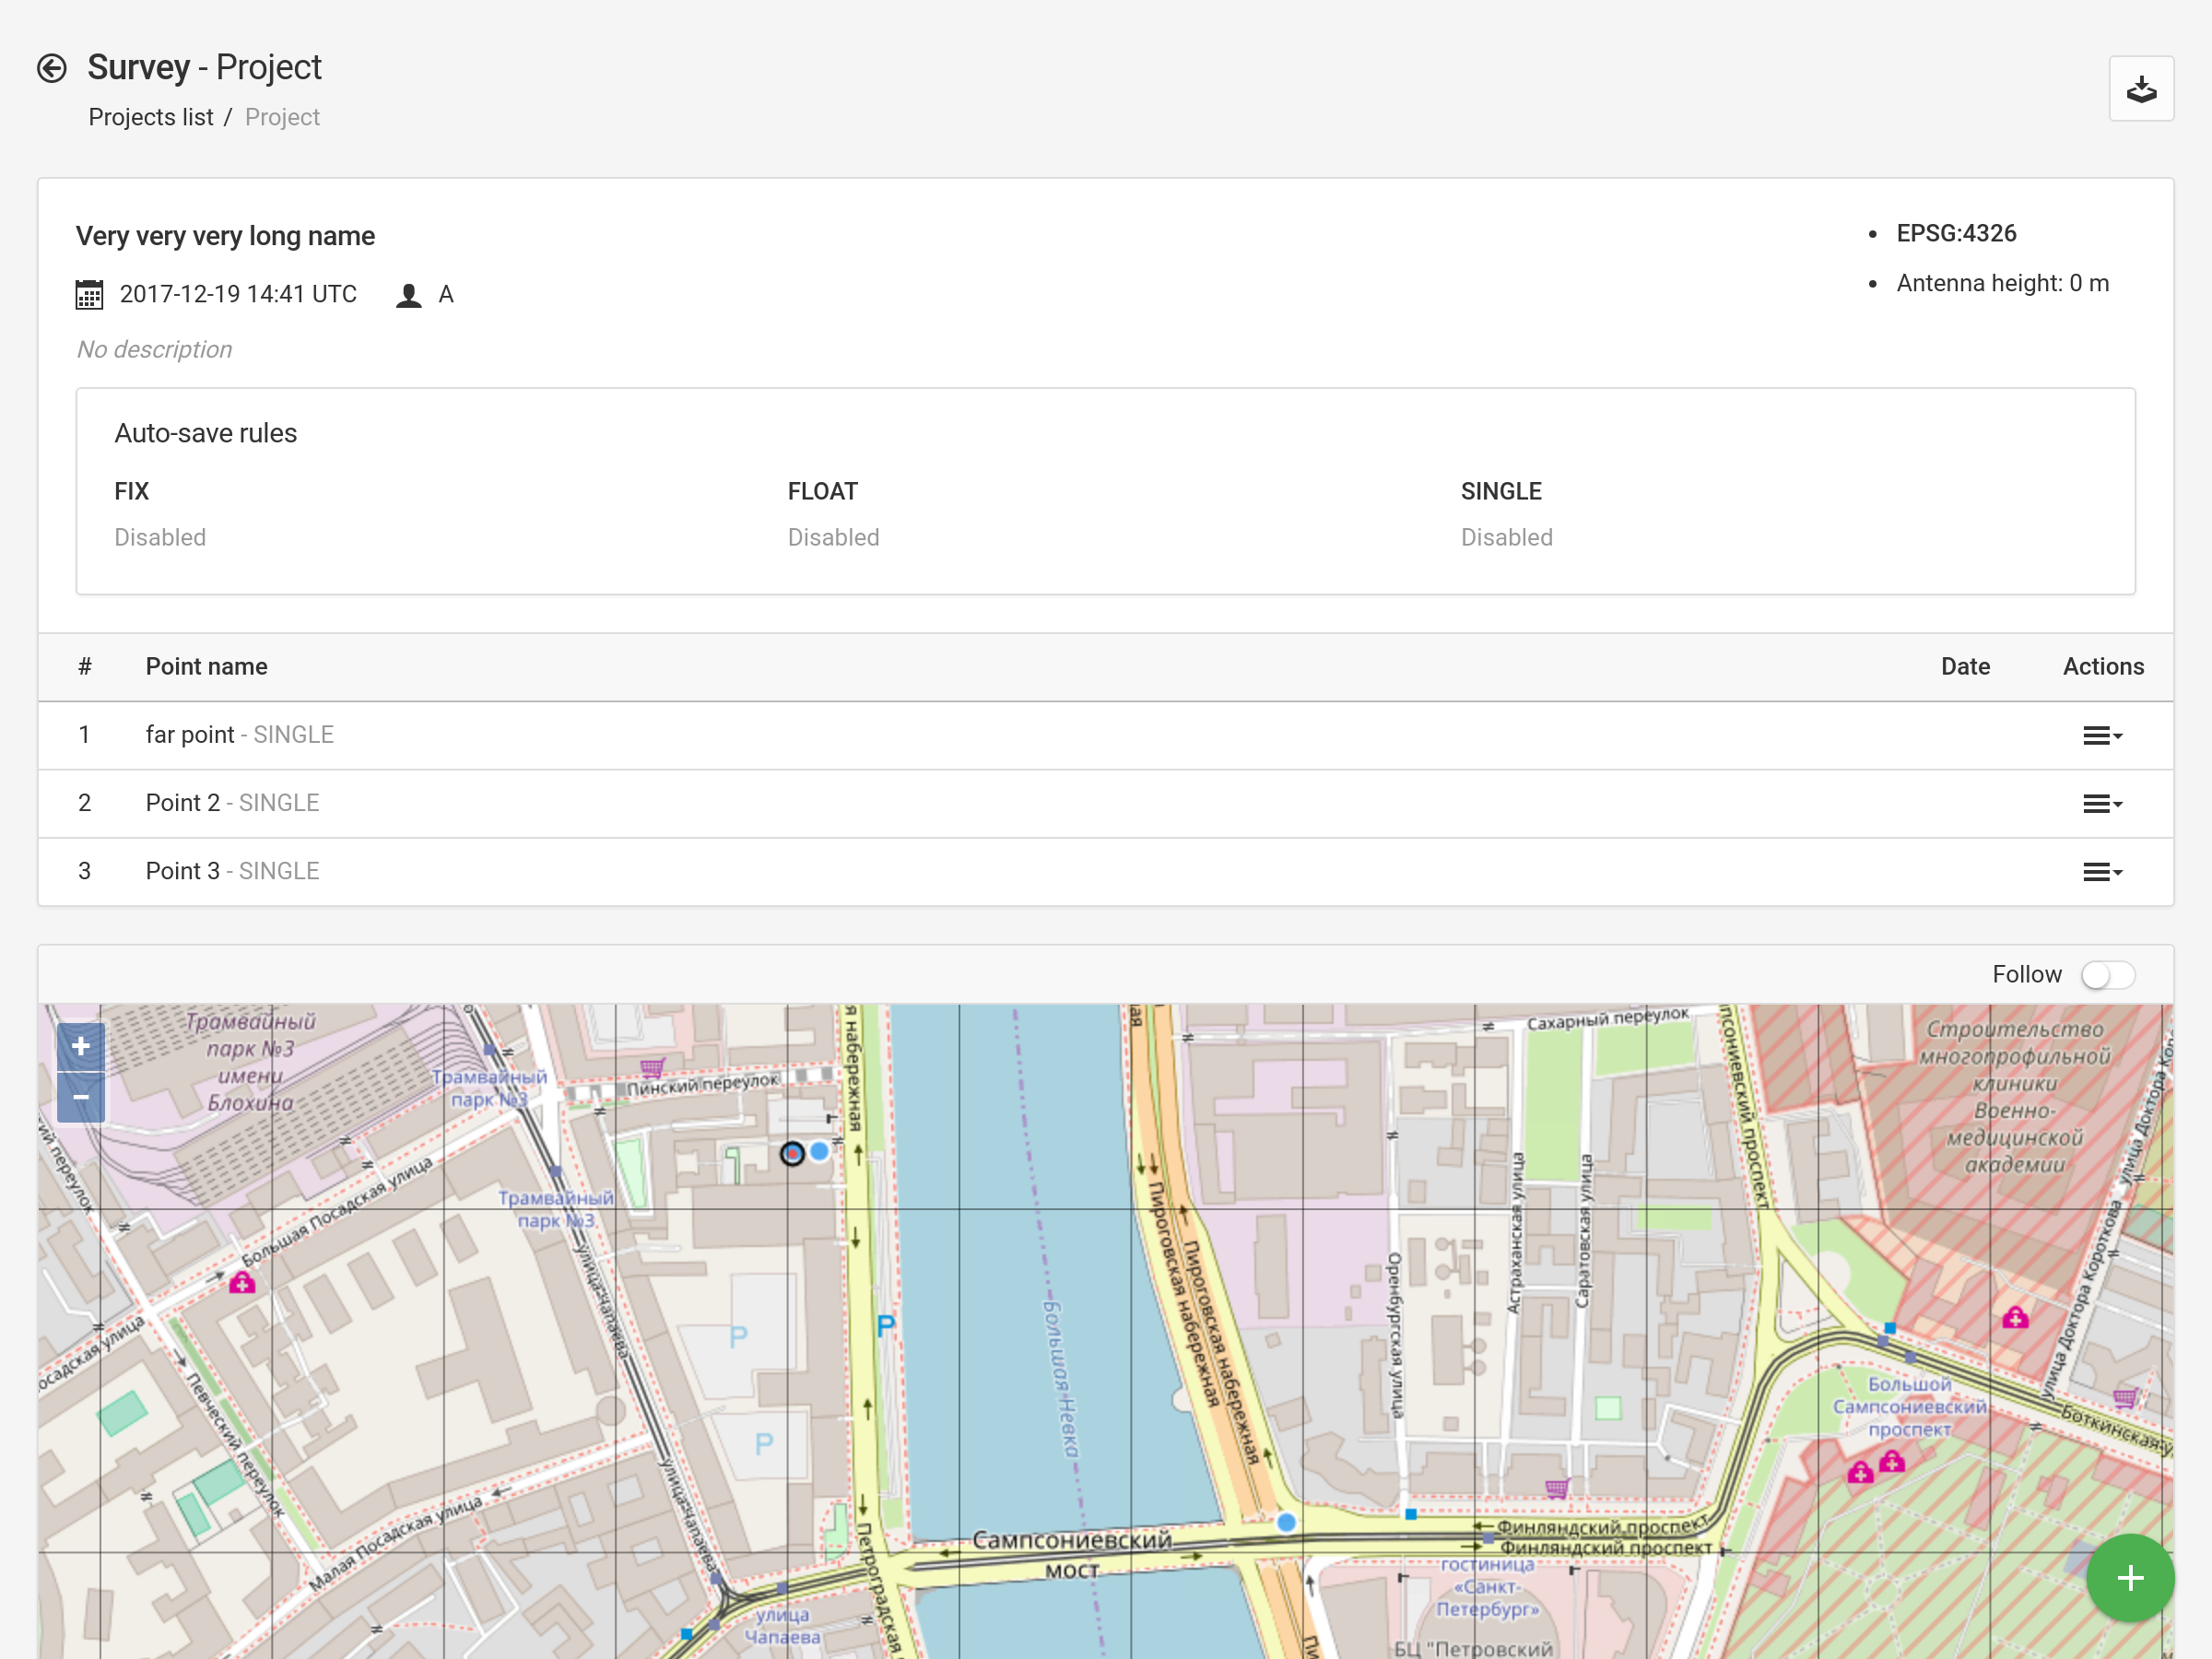
\includegraphics[width=\textwidth]{../img/reachview/survey_content_laptop}
        \end{figure}
      }
      \only<3>{
        \begin{figure}[c]
          \centering
          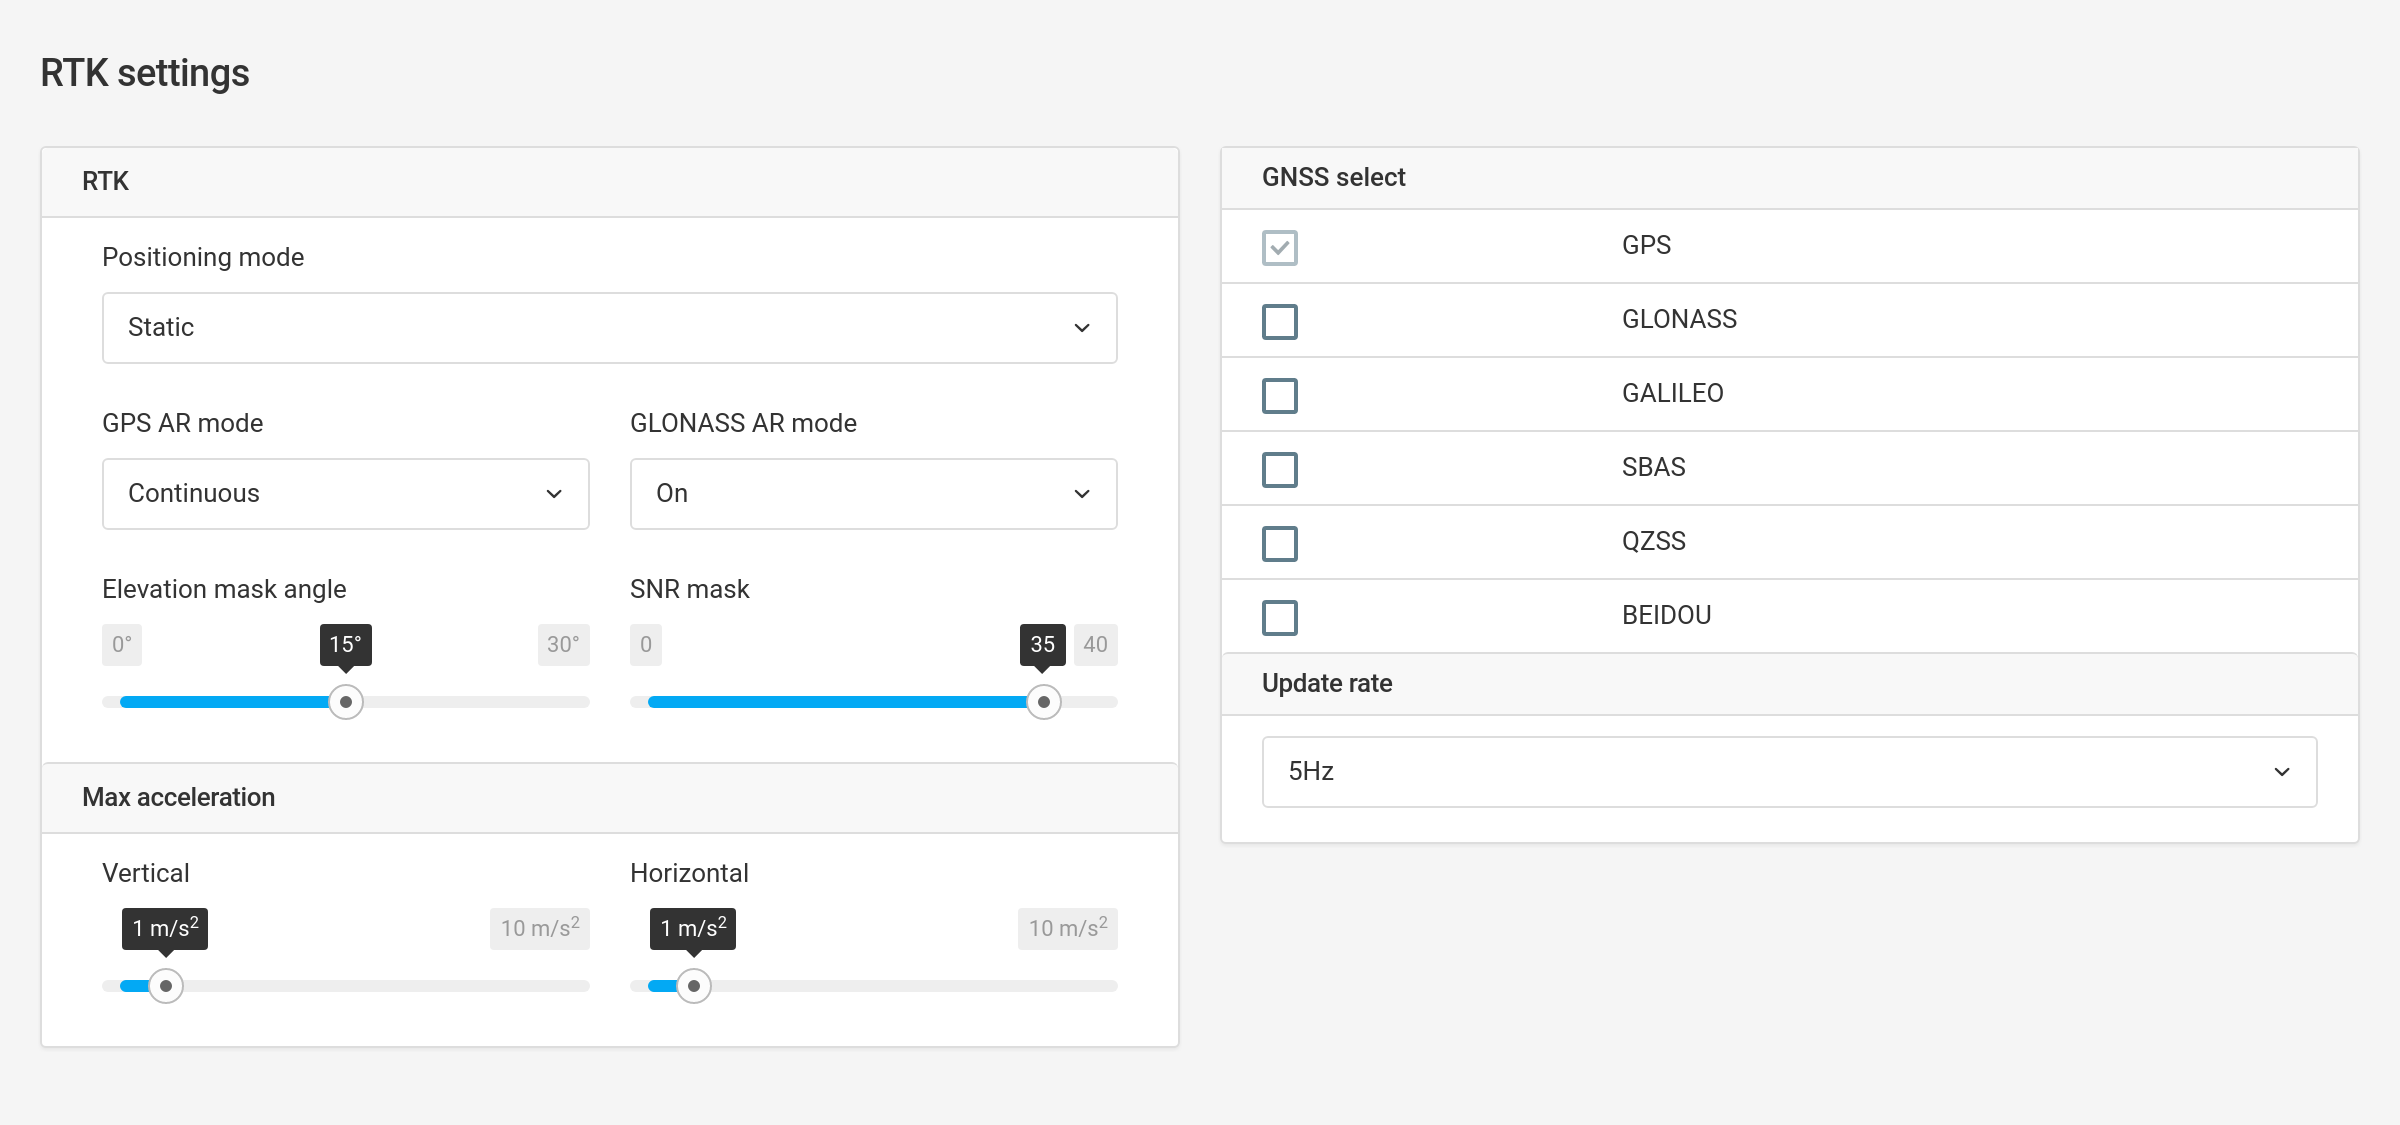
\includegraphics[width=\textwidth]{../img/reachview/rtk-settings_content_laptop}
        \end{figure}
      }
      \only<4>{
        \begin{figure}[c]
          \centering
          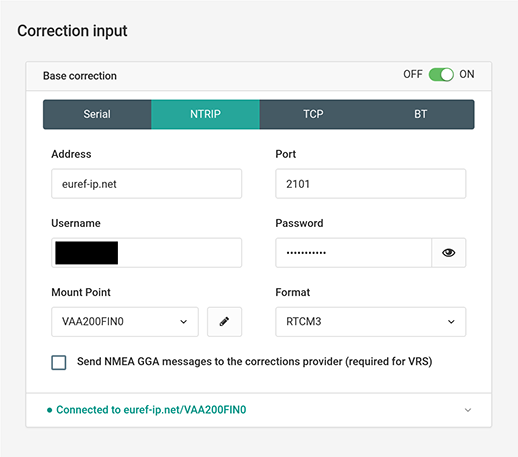
\includegraphics[width=\textwidth]{../img/reachview/correction-input_content_laptop}
        \end{figure}
      }
      \only<5>{
        \begin{figure}[c]
          \centering
          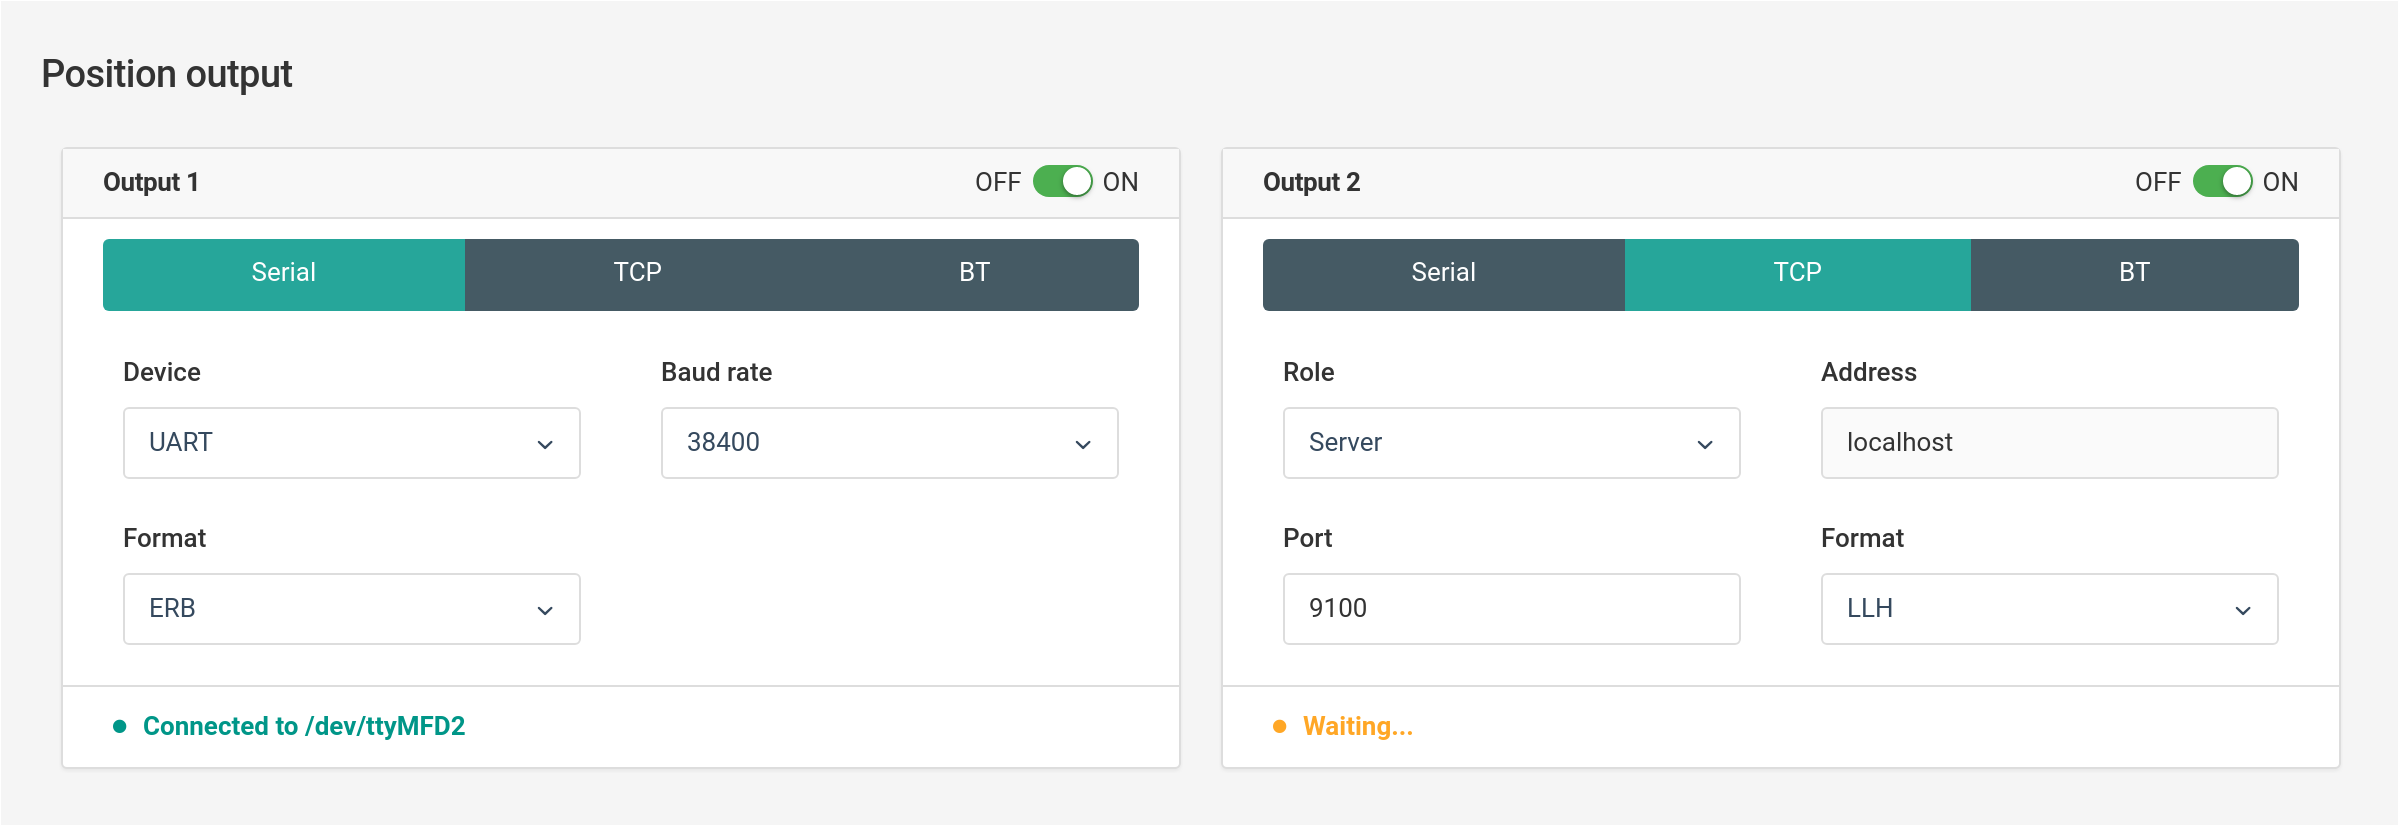
\includegraphics[width=\textwidth]{../img/reachview/position-output_content_laptop}
        \end{figure}
      }
      \only<6>{
        \begin{figure}[c]
          \centering
          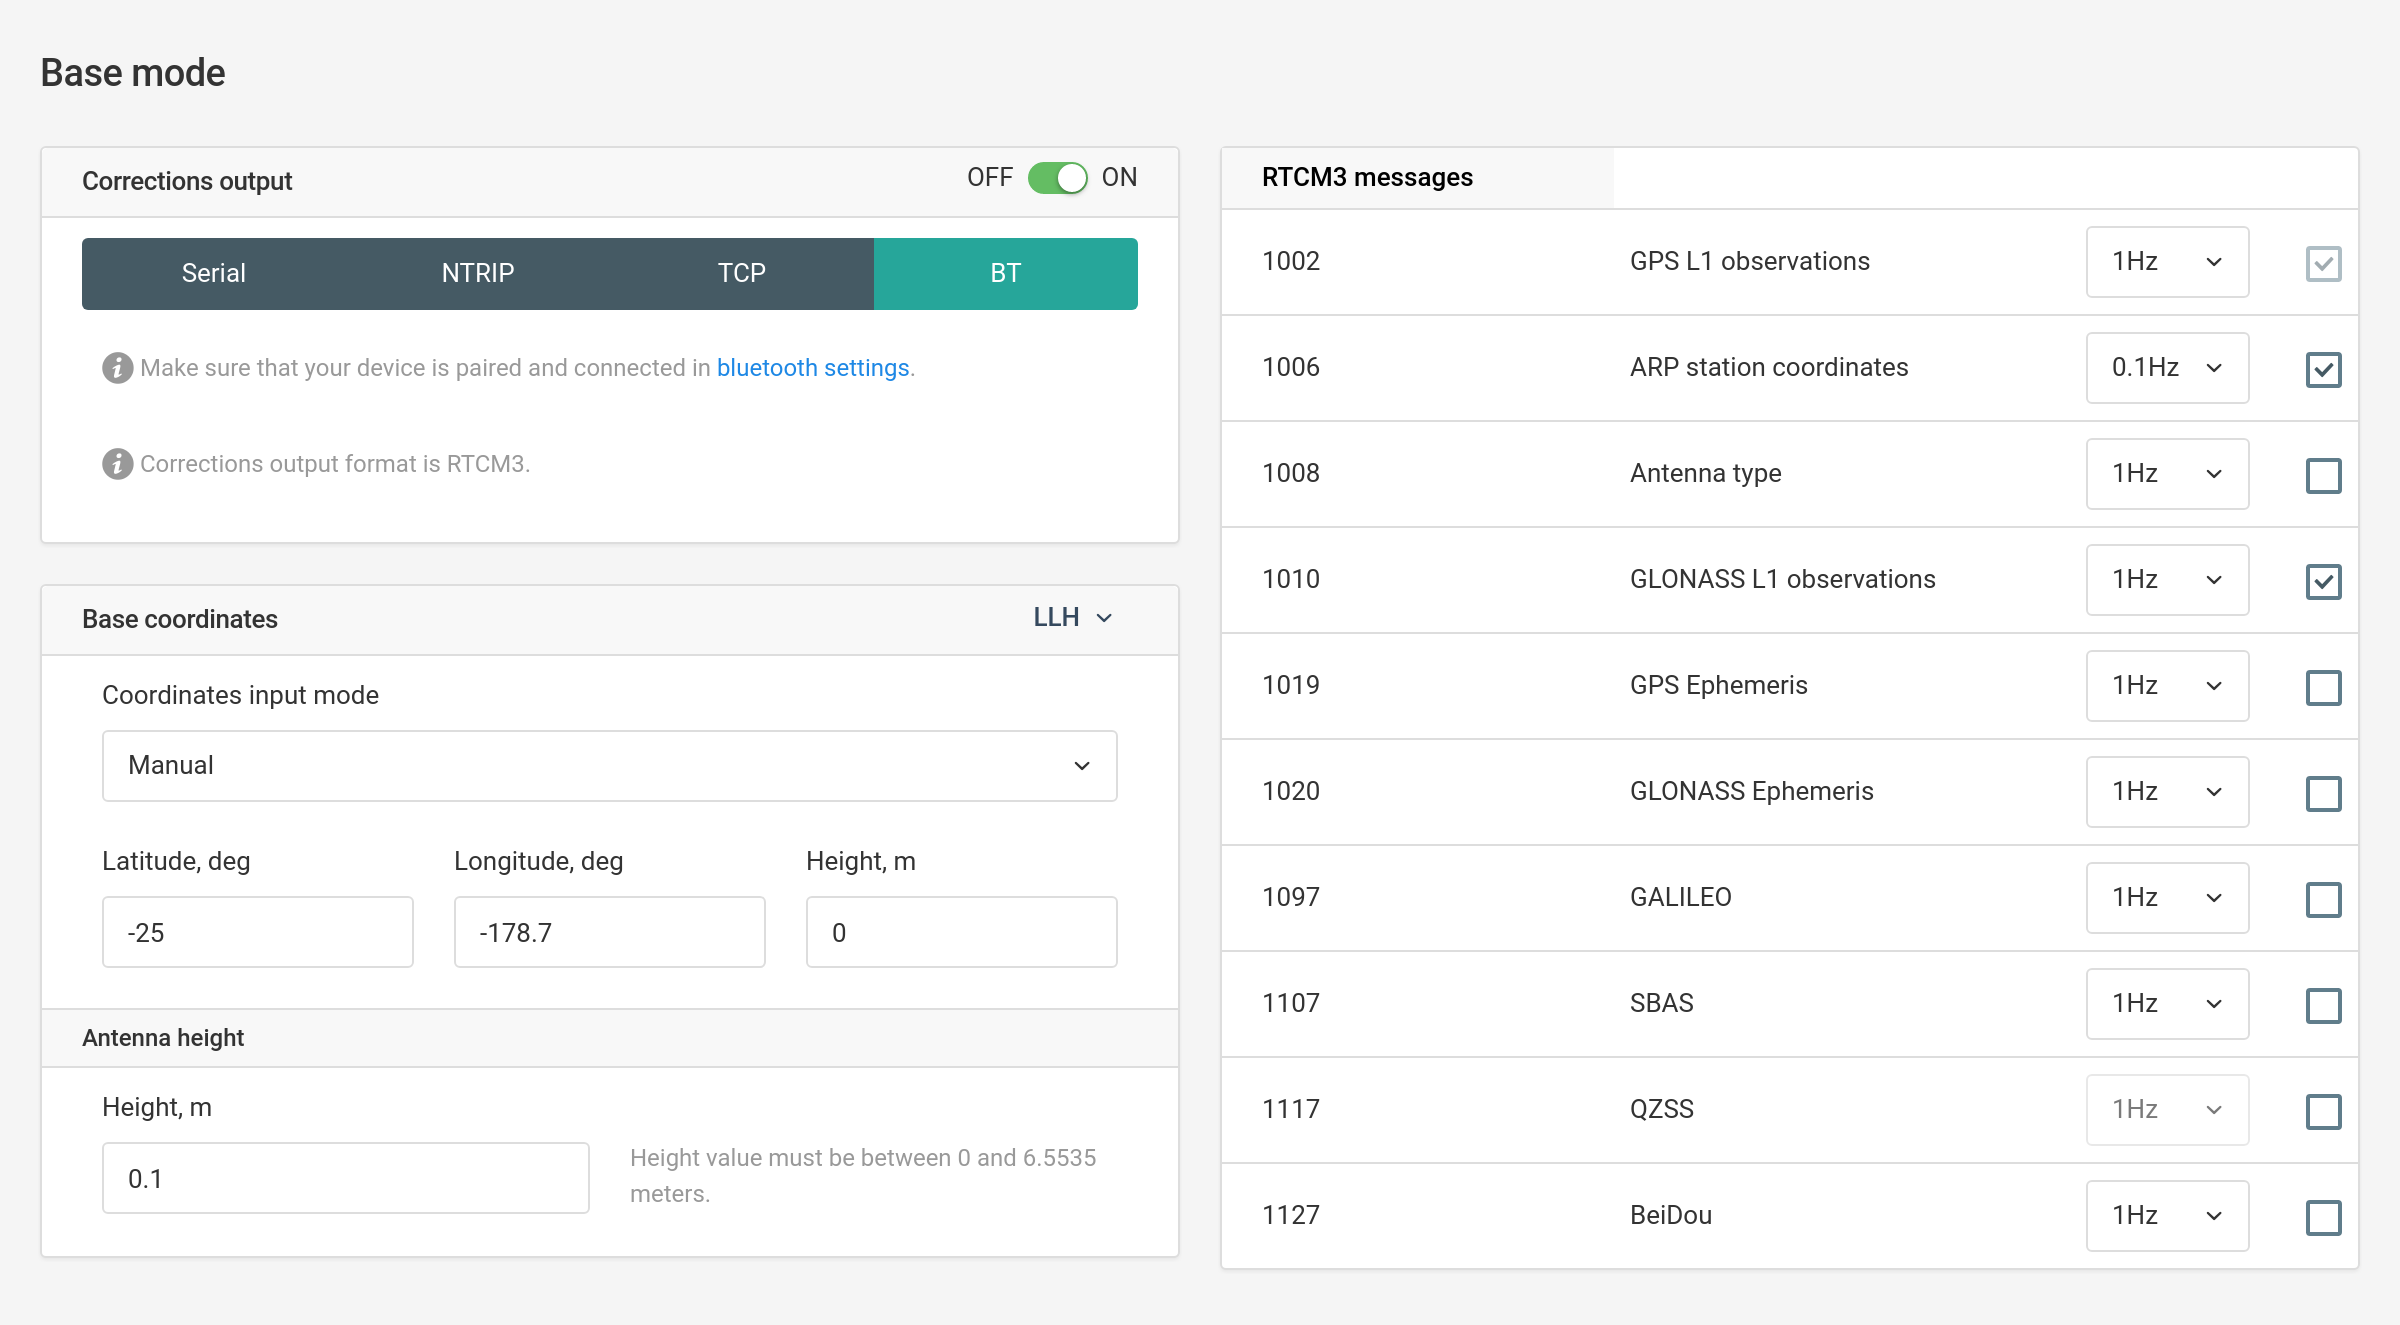
\includegraphics[width=\textwidth]{../img/reachview/base-mode_content_laptop}
        \end{figure}
      }
      \only<7>{
        \begin{figure}[c]
          \centering
          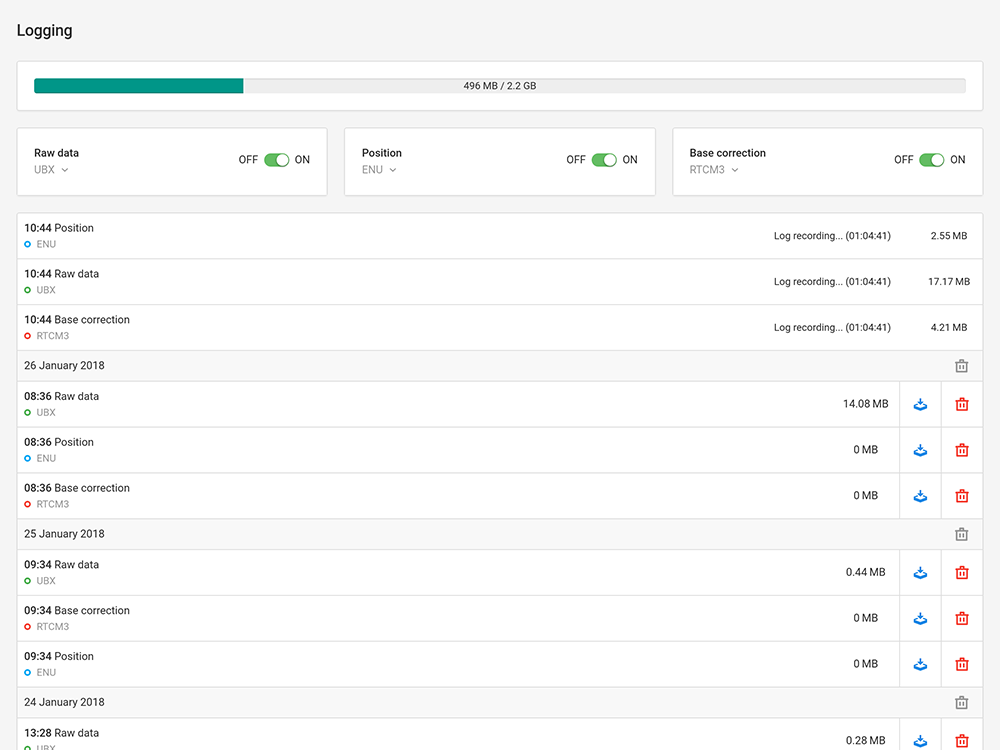
\includegraphics[width=\textwidth]{../img/reachview/logging_content_laptop}
        \end{figure}
      }
      \only<8>{
        \begin{figure}[c]
          \centering
          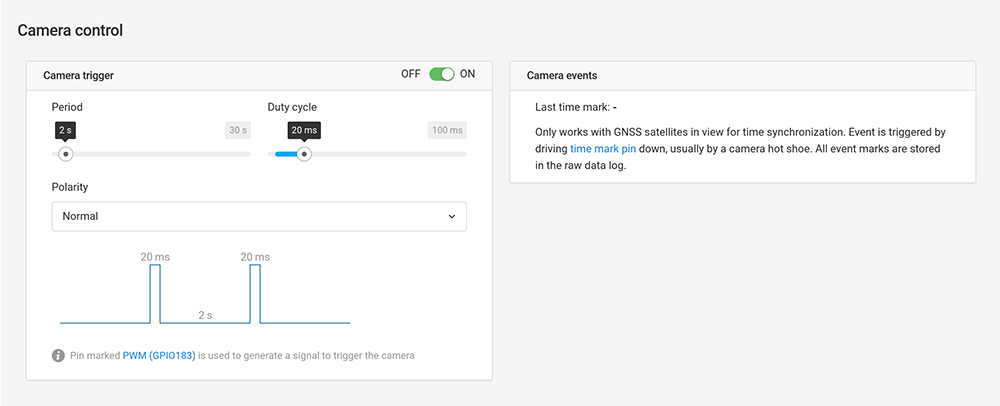
\includegraphics[width=\textwidth]{../img/reachview/camera-control_content_laptop}
        \end{figure}
      }
      \only<9>{
        \begin{figure}[c]
          \centering
          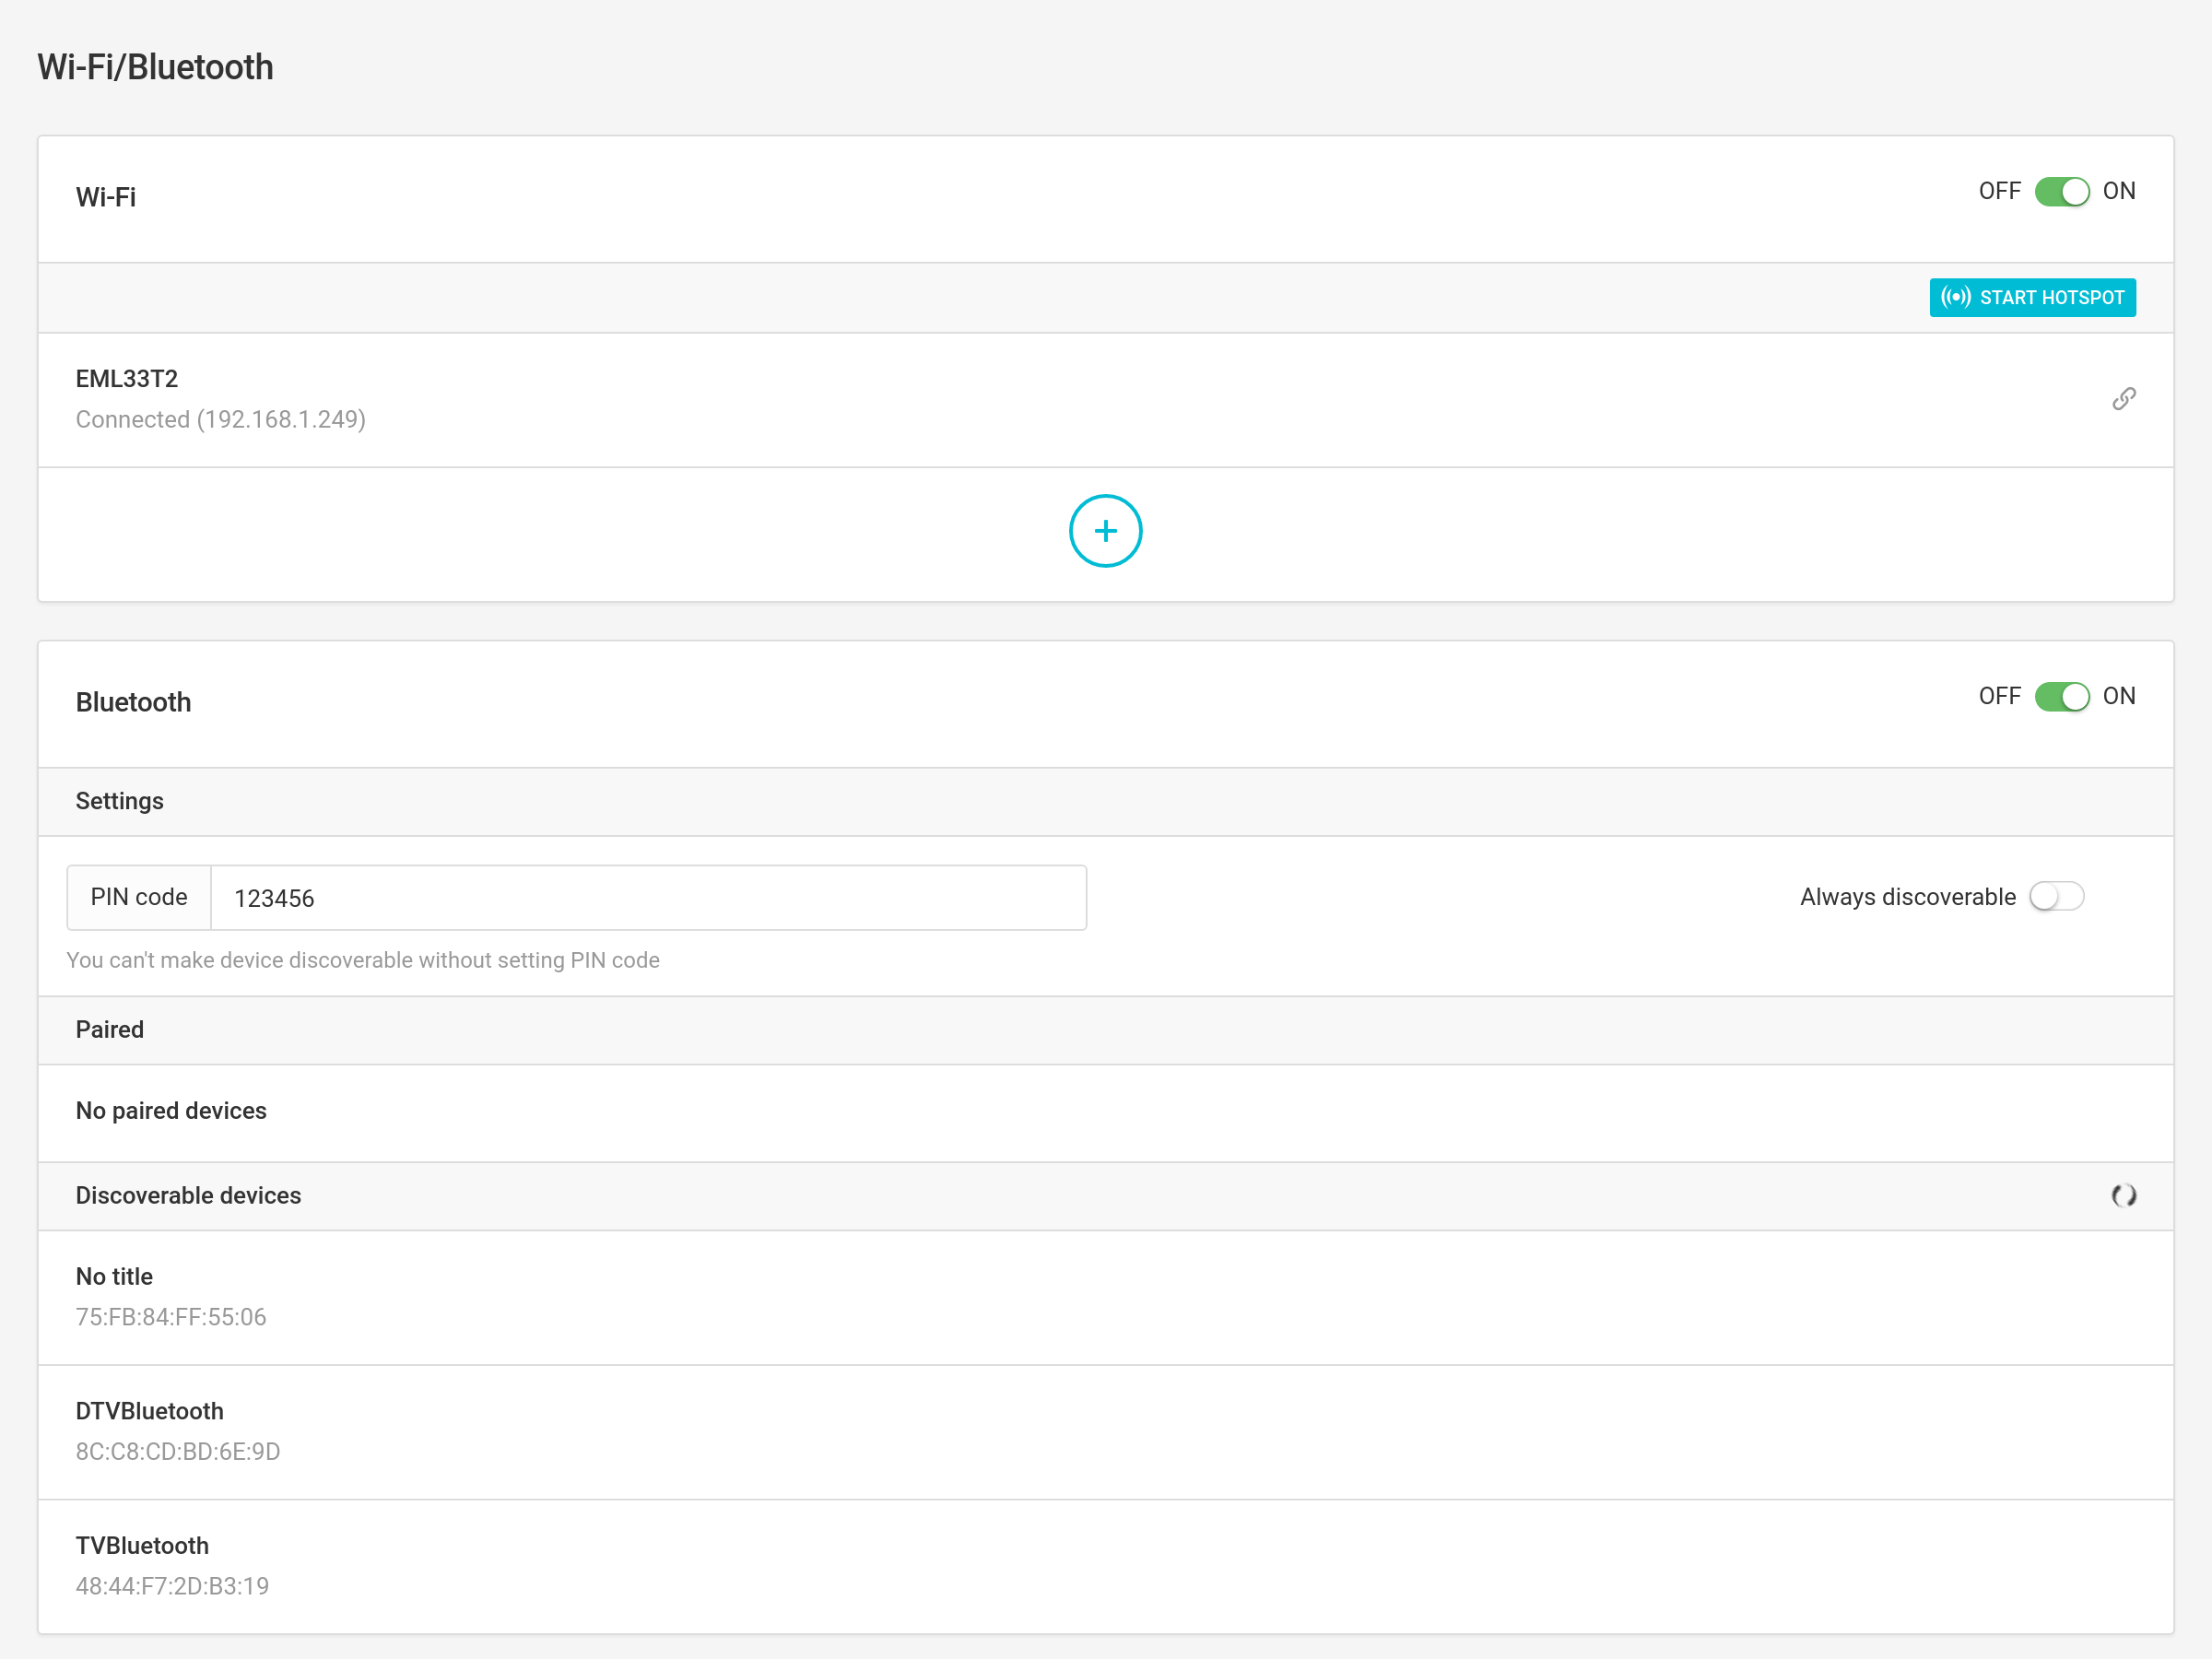
\includegraphics[width=\textwidth]{../img/reachview/wifi-bt_content_laptop}
        \end{figure}
      }
      \only<10>{
        \begin{figure}[c]
          \centering
          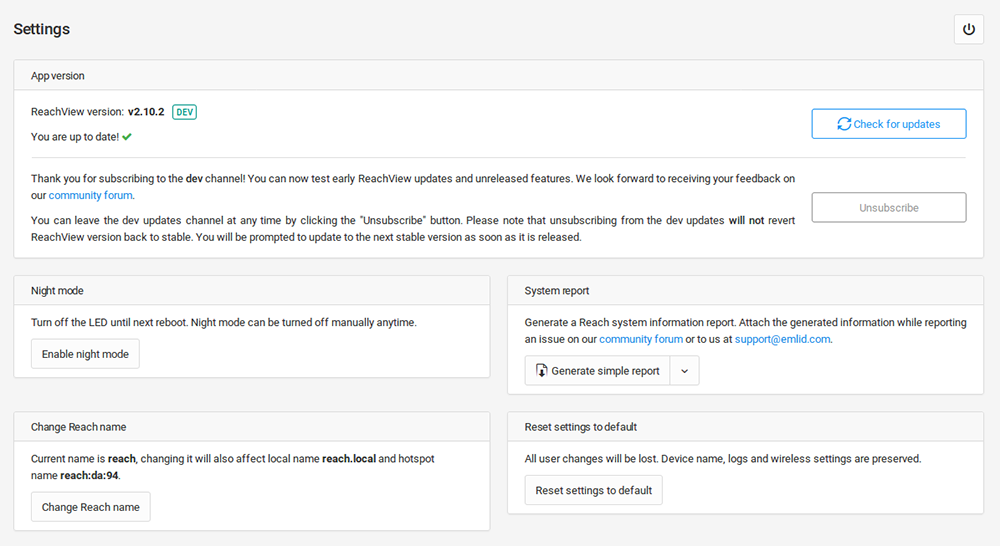
\includegraphics[width=\textwidth]{../img/reachview/settings_content_laptop}
        \end{figure}
      }
    \end{minipage}
  \end{minipage}
\end{frame}


%
% Testing
%
\begin{frame}
  \frametitle{Тестирование приложения}
\end{frame}


%
% Results
%
\begin{frame}
  \frametitle{Результаты}
\end{frame}


%
% The End
%
\begin{frame}[c]
\begin{center}
  \Huge\bfseries
  \color{ifmoblue}{Спасибо за внимание}
\end{center}
\end{frame}

\end{document}
